\documentclass[compress,red]{beamer}
\mode<presentation>
\setbeamertemplate{navigation symbols}{}

\usetheme{Warsaw}


%\hypersetup{pdfpagemode=FullScreen} % makes your presentation go automatically to full screen

% define your own colors:
\definecolor{Red}{rgb}{1,0,0}
\definecolor{Blue}{rgb}{0,0,1}
\definecolor{Green}{rgb}{0,1,0}
\definecolor{magenta}{rgb}{1,0,.6}
\definecolor{lightblue}{rgb}{0,.5,1}
\definecolor{lightpurple}{rgb}{.6,.4,1}
\definecolor{gold}{rgb}{.6,.5,0}
\definecolor{orange}{rgb}{1,0.4,0}
\definecolor{hotpink}{rgb}{1,0,0.5}
\definecolor{newcolor2}{rgb}{.5,.3,.5}
\definecolor{newcolor}{rgb}{0,.3,1}
\definecolor{newcolor3}{rgb}{1,0,.35}
\definecolor{darkgreen1}{rgb}{0, .35, 0}
\definecolor{darkgreen}{rgb}{0, .6, 0}
\definecolor{darkred}{rgb}{.75,0,0}

\xdefinecolor{olive}{cmyk}{0.64,0,0.95,0.4}
\xdefinecolor{purpleish}{cmyk}{0.75,0.75,0,0}


\useoutertheme[subsection=false]{smoothbars}


% include packages
\usepackage{subfigure}
\usepackage{multicol}
\usepackage{amsmath}
\usepackage{epsfig}
\usepackage{graphicx}
\usepackage[all,knot]{xy}
\xyoption{arc}
\usepackage{url}
\usepackage{multimedia}
\usepackage{hyperref}
\usepackage{helvet}
\usepackage[polish,english]{babel}
\usepackage[utf8]{inputenc}
\usepackage{multirow}
\usepackage{amsfonts}
%%%%%%%%%%%%5
%\usepackage{geometry}
%\geometry{verbose,letterpaper}
%\usepackage{movie15}
%\usepackage{hyperref}
%%%%%%%

% greetings, introduce yourself

\newcommand{\tickYes}{\checkmark}
 \usepackage{pifont}
 \newcommand{\tickNo}{\hspace{1pt}\ding{55}}
%  
\includegraphics[height=5cm]{fig/WRlogo.ps}


\title[White Rabbit Network\hspace{2em}\insertframenumber/\inserttotalframenumber]
{White Rabbit Network\\ Status and Plans}

\institute{
\begin{columns}[c]
  \column{.5\textwidth}
   \begin{center}
    Hardware and Timing Section\\
    CERN
   \end{center}
  \column{.5\textwidth}
   \begin{center}    
    Bel Division \\
    GSI
   \end{center}
  \end{columns}
}
\author{
Maciej Lipi\'{n}ski~~~~~~~~~~~~~~~~~~~~~~~~~~~~~~~~~~Cesar Prados %, T.W\l{}ostowski, J.Serrano, P.Alvarez
}
\date{March 2012}



% \institute%[Universities of Somewhere and Elsewhere] % (optional, but mostly needed)
% {
%   \begin{center}
%     BE-CO-HT\\
%     CERN, Geneva,\\
%     Switzerland\\
%   \end{center}
% }

\pgfdeclareimage[height=0.6cm]{wr-logo}{../../figures/logo/WRlogo.ps}
\logo{\pgfuseimage{wr-logo}}
\AtBeginSection[]
% {
%   \begin{frame}<beamer>{Outline}
%     \tableofcontents[currentsection]
%   \end{frame}
% }

\begin{document}

\frame{\titlepage}
%%%%%%%%%%%%%%%%%%%%%%%%%%%%%%%%%%%%%%%%%%%%%%%%%%%%%%%%%%%%%%%%%%%%%%%%%%%%%%%%%%%%%%%%%%%%%%%%%%%%
% \begin{frame}<beamer>{Outline}
% 
%     \tableofcontents %[currentsection]
% 
% \end{frame}
%%%%%%%%%%%%%%%%%%%%%%%%%%%%%%%%%%%%%%%%%%%%%%%%%%%%%%%%%%%%%%%%%%%%%%%%%%%%%%%%%%%%%%%%%%%%%%%%%%%%
\section{Introduction}
\subsection{}
%%%%%%%%%%%%%%%%%%%%%%%%%%%%%%%%%%%%%%%%%%%%%%%%%%%%%%%%%%%%%%%%%%%%%%%%%%%%%%%%%%%%%%%%%%%%%%%%%%%%
\begin{frame}{White Rabbit Network}

%   \begin{columns}[c]
%   \column{.43\textwidth}
%     \begin{itemize}
%       \item WR Switches and WR Nodes
%       \item Two service:
%       \begin{itemize}
% 	\item Time distribution
% 	\item Data distribution
%       \end{itemize}
%       \item {\bf High reliability required}
%     \end{itemize}
%   \column{.57\textwidth}
% 
%       \begin{center}
% 	\includegraphics[height=6.5cm]{fig/WR_funny_network.ps}
% 	\includegraphics[height=6.5cm]{fig/sub_domains.ps}
%       \end{center}    
% 
%   \end{columns}
  

      \begin{center}
	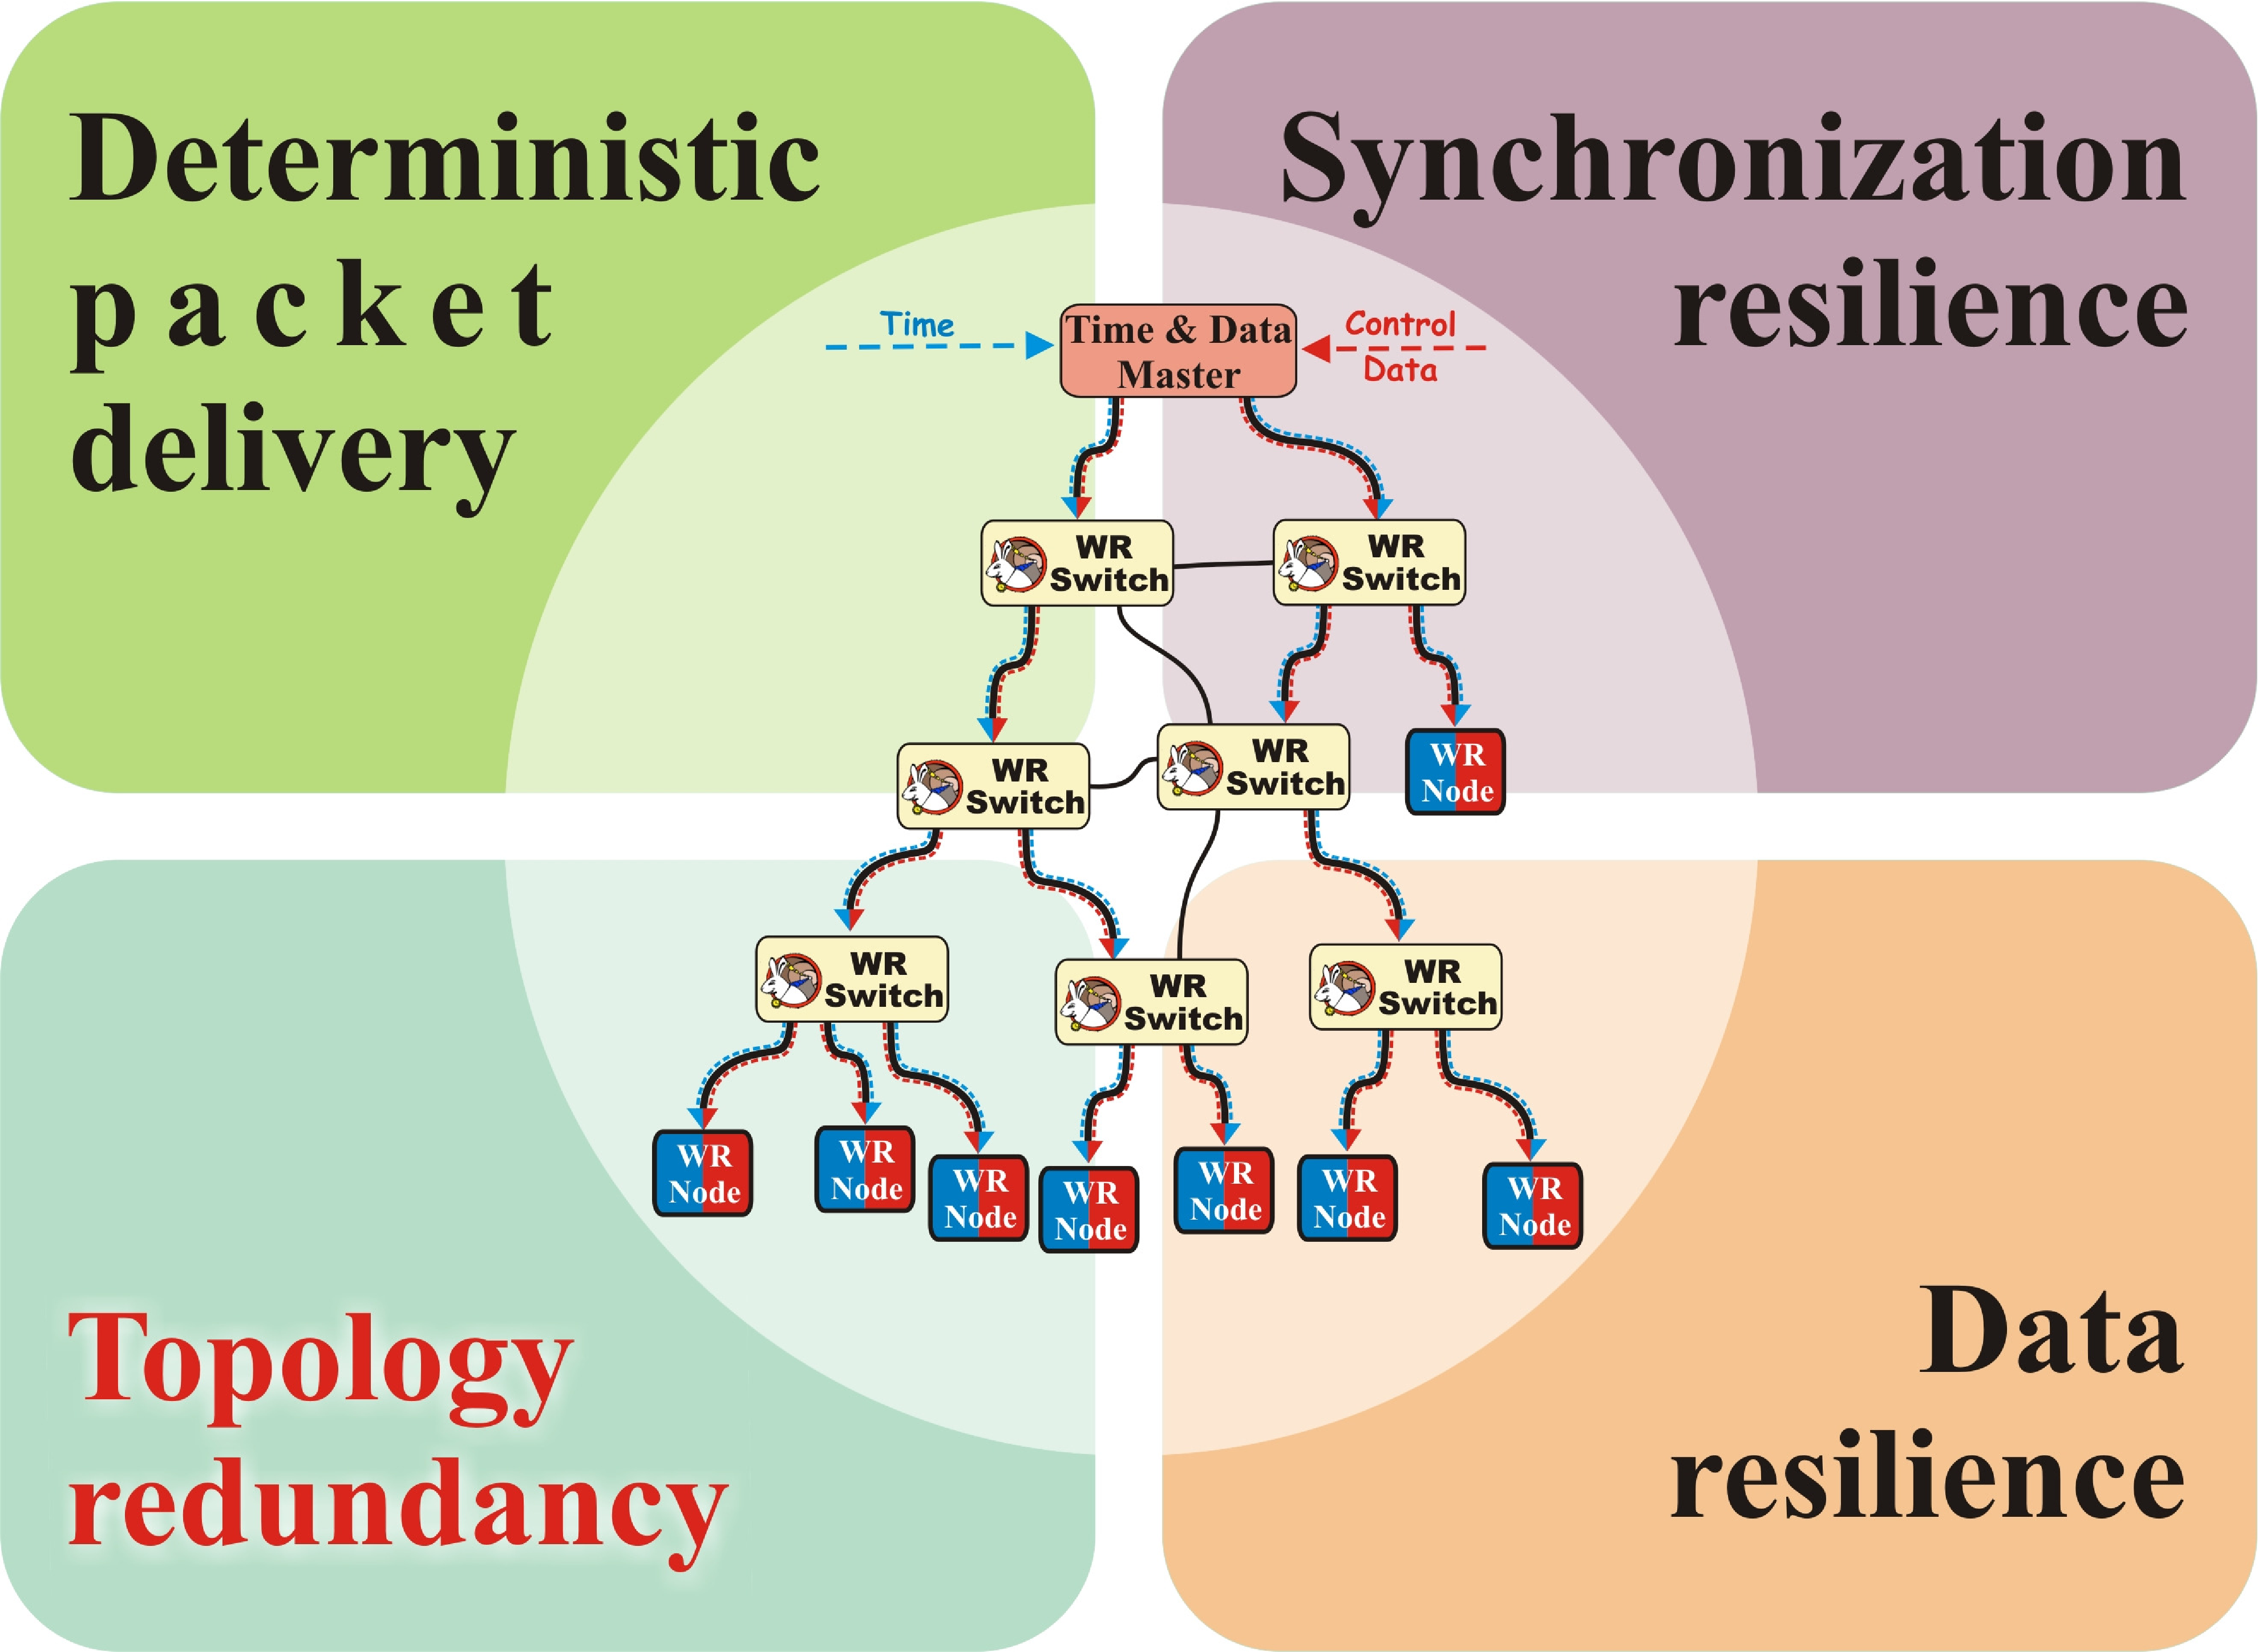
\includegraphics[width=.9\textwidth]{../../figures/robustness/sub_domains-old.ps}
      \end{center}    


\end{frame}
%%%%%%%%%%%%%%%%%%%%%%%%%%%%%%%%%%%%%%%%%%%%%%%%%%%%%%%%%%%%%%%%%%%%%%%%%%%%%%%%%%%%%%%%%%%%%%%%%%%%
% \section{Synchronization}
% \subsection{}
%%%%%%%%%%%%%%%%%%%%%%%%%%%%%%%%%%%%%%%%%%%%%%%%%%%%%%%%%%%%%%%%%%%%%%%%%%%%%%%%%%%%%%%%%%%%%%%%%%%%
\begin{frame}<beamer>{Outline}

    \tableofcontents %[currentsection]

\end{frame}
%%%%%%%%%%%%%%%%%%%%%%%%%%%%%%%%%%%%%%%%%%%%%%%%%%%%%%%%%%%%%%%%%%%%%%%%%%%%%%%%%%%%%%%%%%%%%%%%%%%%
\section{Synchronization}
\subsection{}
%%%%%%%%%%%%%%%%%%%%%%%%%%%%%%%%%%%%%%%%%%%%%%%%%%%%%%%%%%%%%%%%%%%%%%%%%%%%%%%%%%%%%%%%%%%%%%%%%%%%
\begin{frame}{Time Distribution}

  \begin{columns}[c]
  \column{.7\textwidth}

  \begin{itemize}
    \item Network-wide {\bf sub-ns}~synchronization
    \vspace{0.3cm}
    \item Constant performance in:
	\begin{itemize}
	  \item {\bf stable} conditions
	  \item {\bf transient} conditions
	\end{itemize}
    \vspace{0.3cm}
    \item Support for network redundancy
    \begin{itemize}
      \item WRPTP 
\includegraphics[width=.5cm]{../../figures/misc/big-tick.ps}  (possibly further improve)
      \item Hardware 
\includegraphics[width=.5cm]{../../figures/misc/underconstruction.ps}
    \end{itemize}
  \end{itemize}

  \column{.3\textwidth}

      \begin{center}
	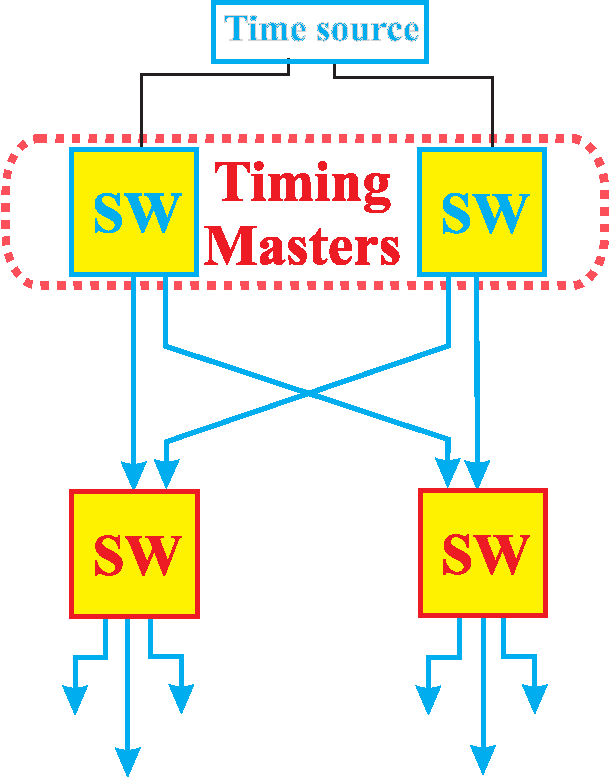
\includegraphics[width=1.1\textwidth]{../../figures/robustness/WRPTPmodif_0.eps}
      \end{center}  
    

  \end{columns}

\end{frame}
%%%%%%%%%%%%%%%%%%%%%%%%%%%%%%%%%%%%%%%%%%%%%%%%%%%%%%%%%%%%%%%%%%%%%%%%%%%%%%%%%%%%%%%%%%%%%%%%%%%%
%\section{Synchronization}
%\subsection{}
%%%%%%%%%%%%%%%%%%%%%%%%%%%%%%%%%%%%%%%%%%%%%%%%%%%%%%%%%%%%%%%%%%%%%%%%%%%%%%%%%%%%%%%%%%%%%%%%%%%%
\begin{frame}{Time Distribution}

  \begin{columns}[c]
  \column{.7\textwidth}

  \begin{itemize}
    \item Network-wide {\bf sub-ns}~synchronization
    \vspace{0.3cm}
    \item Constant performance in:
	\begin{itemize}
	  \item {\bf stable} conditions
	  \item {\bf transient} conditions
	\end{itemize}
    \vspace{0.3cm}
    \item Support for network redundancy
    \begin{itemize}
      \item WRPTP 
\includegraphics[width=.5cm]{../../figures/misc/big-tick.ps}  (possibly further improve)
      \item Hardware 
\includegraphics[width=.5cm]{../../figures/misc/underconstruction.ps}
    \end{itemize}
  \end{itemize}

  \column{.3\textwidth}

      \begin{center}
	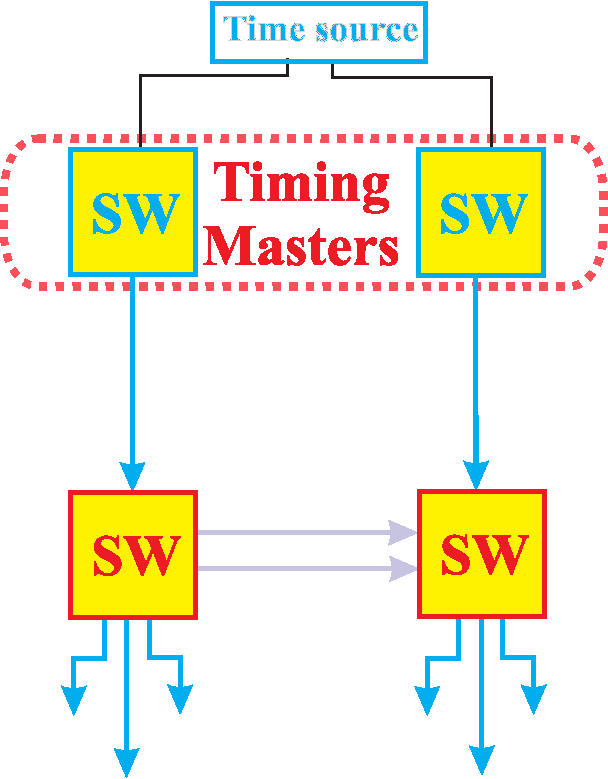
\includegraphics[width=1.1\textwidth]{../../figures/robustness/WRPTPmodif_1.eps}
      \end{center}  
    

  \end{columns}

\end{frame}
%%%%%%%%%%%%%%%%%%%%%%%%%%%%%%%%%%%%%%%%%%%%%%%%%%%%%%%%%%%%%%%%%%%%%%%%%%%%%%%%%%%%%%%%%%%%%%%%%%%%
%\section{Synchronization}
%\subsection{}
%%%%%%%%%%%%%%%%%%%%%%%%%%%%%%%%%%%%%%%%%%%%%%%%%%%%%%%%%%%%%%%%%%%%%%%%%%%%%%%%%%%%%%%%%%%%%%%%%%%%
\begin{frame}{Time Distribution}

  \begin{columns}[c]
  \column{.7\textwidth}

  \begin{itemize}
    \item Network-wide {\bf sub-ns}~synchronization
    \vspace{0.3cm}
    \item Constant performance in:
	\begin{itemize}
	  \item {\bf stable} conditions
	  \item {\bf transient} conditions
	\end{itemize}
    \vspace{0.3cm}
    \item Support for network redundancy
    \begin{itemize}
      \item WRPTP 
\includegraphics[width=.5cm]{../../figures/misc/big-tick.ps}  (possibly further improve)
      \item Hardware 
\includegraphics[width=.5cm]{../../figures/misc/underconstruction.ps}
    \end{itemize}
  \end{itemize}

  \column{.3\textwidth}

      \begin{center}
	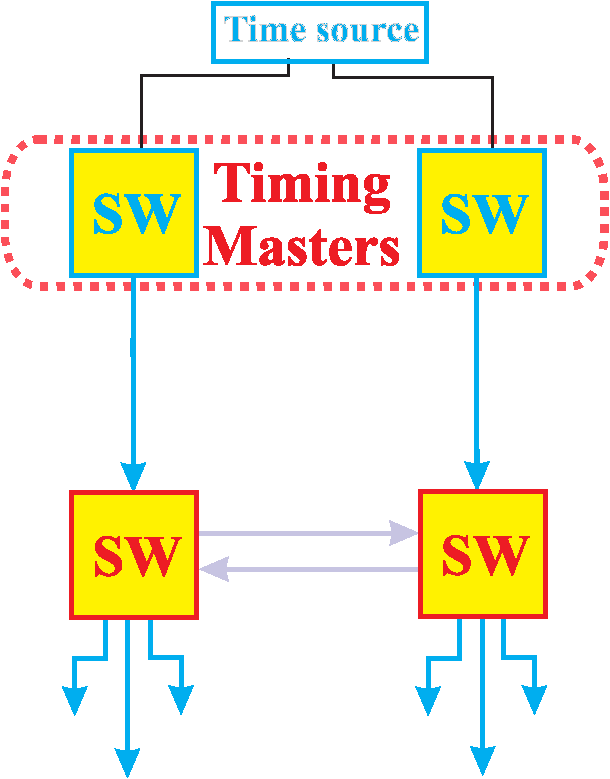
\includegraphics[width=1.1\textwidth]{../../figures/robustness/WRPTPmodif_2.eps}
      \end{center}  
    

  \end{columns}

\end{frame}
%%%%%%%%%%%%%%%%%%%%%%%%%%%%%%%%%%%%%%%%%%%%%%%%%%%%%%%%%%%%%%%%%%%%%%%%%%%%%%%%%%%%%%%%%%%%%%%%%%%%
\section{Determinism}
\subsection{}
%%%%%%%%%%%%%%%%%%%%%%%%%%%%%%%%%%%%%%%%%%%%%%%%%%%%%%%%%%%%%%%%%%%%%%%%%%%%%%%%%%%%%%%%%%%%%%%%%%%%
\begin{frame}{Deterministic data delivery}

%\begin{columns}[c]
  %\column{.5\textwidth}

    \begin{block}{{\bf Special Traffic ({\bf optional})}}
    \begin{itemize}
      \item Priority 7 (broadcast)  
      \item Quality of Service (QoS)
      \item Determinism of data delivery
    \end{itemize}
    \end{block}


%  \column{.5\textwidth}

%    \vspace{3cm}
\hspace{4cm}
    \begin{block}{ {\bf Normal Traffic}}
    \begin{itemize}
      \item Any non priority 7 traffic 
      \item Less stringent determinism of data delivery
    \end{itemize}   
    \end{block}

%  \end{columns}

%   \begin{itemize}
%     \item Special Traffic ({\bf optional})
%     \begin{itemize}
%       \item Priority 7 (broadcast)  
%       \item Quality of Service (QoS)
%       \item Determinism data delivery
%     \end{itemize}
%     \item Standard Traffic
%     \begin{itemize}
%       \item Any non priority 7 traffic 
%       \item Less stringent deterministic behavior
%     \end{itemize}
% 
%   \end{itemize}

\end{frame}

%%%%%%%%%%%%%%%%%%%%%%%%%%%%%%%%%%%%%%%%%%%%%%%%%%%%%%%%%%%%%%%%%%%%%%%%%%%%%%%%%%%%%%%%%%%%%%%%%%%%
% \section{Data Distribution}
 %\subsection{Quality of Service}
%%%%%%%%%%%%%%%%%%%%%%%%%%%%%%%%%%%%%%%%%%%%%%%%%%%%%%%%%%%%%%%%%%%%%%%%%%%%%%%%%%%%%%%%%%%%%%%%%%%%
\begin{frame}{Quality of Service (WR Switch)}

  \begin{itemize}
    \item Cut-through 
\includegraphics[width=.5cm]{../../figures/misc/big-tick.ps}
    \item Separate resources for Special Traffic 
\includegraphics[width=.5cm]{../../figures/misc/underconstruction.ps}
    \item Output queuing 
\includegraphics[width=.5cm]{../../figures/misc/underconstruction.ps}
    \item Switch firmware optimization (SWcore + RTU) 
\includegraphics[width=.5cm]{../../figures/misc/underconstruction.ps}
  \end{itemize}

\end{frame}

%%%%%%%%%%%%%%%%%%%%%%%%%%%%%%%%%%%%%%%%%%%%%%%%%%%%%%%%%%%%%%%%%%%%%%%%%%%%%%%%%%%%%%%%%%%%%%%%%%%%
\section{Data}
\subsection{}
%%%%%%%%%%%%%%%%%%%%%%%%%%%%%%%%%%%%%%%%%%%%%%%%%%%%%%%%%%%%%%%%%%%%%%%%%%%%%%%%%%%%%%%%%%%%%%%%%%%%
\begin{frame}{Forward Error Correction}

  \begin{itemize}
    \item Well-researched, concepts agreed
    \item Encoder 
\includegraphics[width=.5cm]{../../figures/misc/big-tick.ps}  not optimized for resources
    \item Decoder 
\includegraphics[width=.5cm]{../../figures/misc/underconstruction.ps}~~(MSc thesis):
    \begin{itemize}
      \item Hardware-accelerated LM32
      \item Eventually to be encoder-decoder
    \end{itemize}

  \end{itemize}

      \begin{center}
	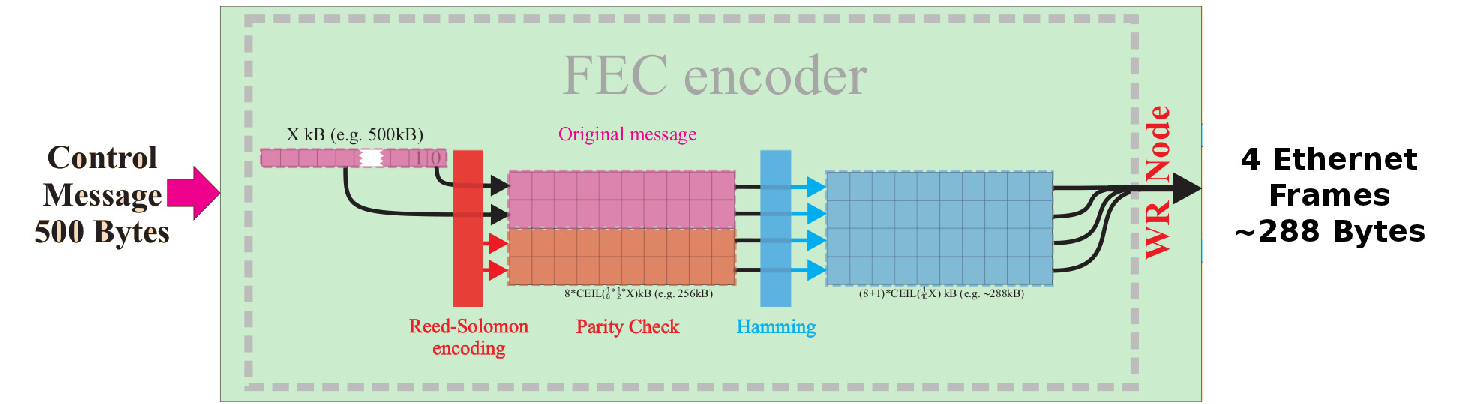
\includegraphics[width=.9\textwidth]{../../figures/robustness/FEC.v2.ps}
      \end{center}  

\end{frame}

%%%%%%%%%%%%%%%%%%%%%%%%%%%%%%%%%%%%%%%%%%%%%%%%%%%%%%%%%%%%%%%%%%%%%%%%%%%%%%%%%%%%%%%%%%%%%%%%%%%%
%\section{Data}
%\subsection{}
%%%%%%%%%%%%%%%%%%%%%%%%%%%%%%%%%%%%%%%%%%%%%%%%%%%%%%%%%%%%%%%%%%%%%%%%%%%%%%%%%%%%%%%%%%%%%%%%%%%%
\begin{frame}{FEC: Linear Code and 8b/10b I}

  \begin{itemize}
    \item The FEC scheme is \textbf{Linear Code} for the Binary Erasure
    Channel and a \textbf{Block Code} for the Packet Erasure Channel. 
    \item The numbers told us that we need to repair just a bit... Hamming was the option.
    \item Gigabit Ethernet uses \textbf{8b/10b} in the physical layer. 
    \item One bit error in a 10 bits encoded code word may result in a multi-bit
    error $>2$ $\rightarrow$
    \textbf{Hamming is not enough!}.
    \item The best Linear Code able to recover 4 bit error and detect up to 8 is
    the \textbf{Golay Code Family}.
  \end{itemize}
\end{frame}

\begin{frame}{FEC: Linear Code and 8b/10b II}
 
 \begin{center}
 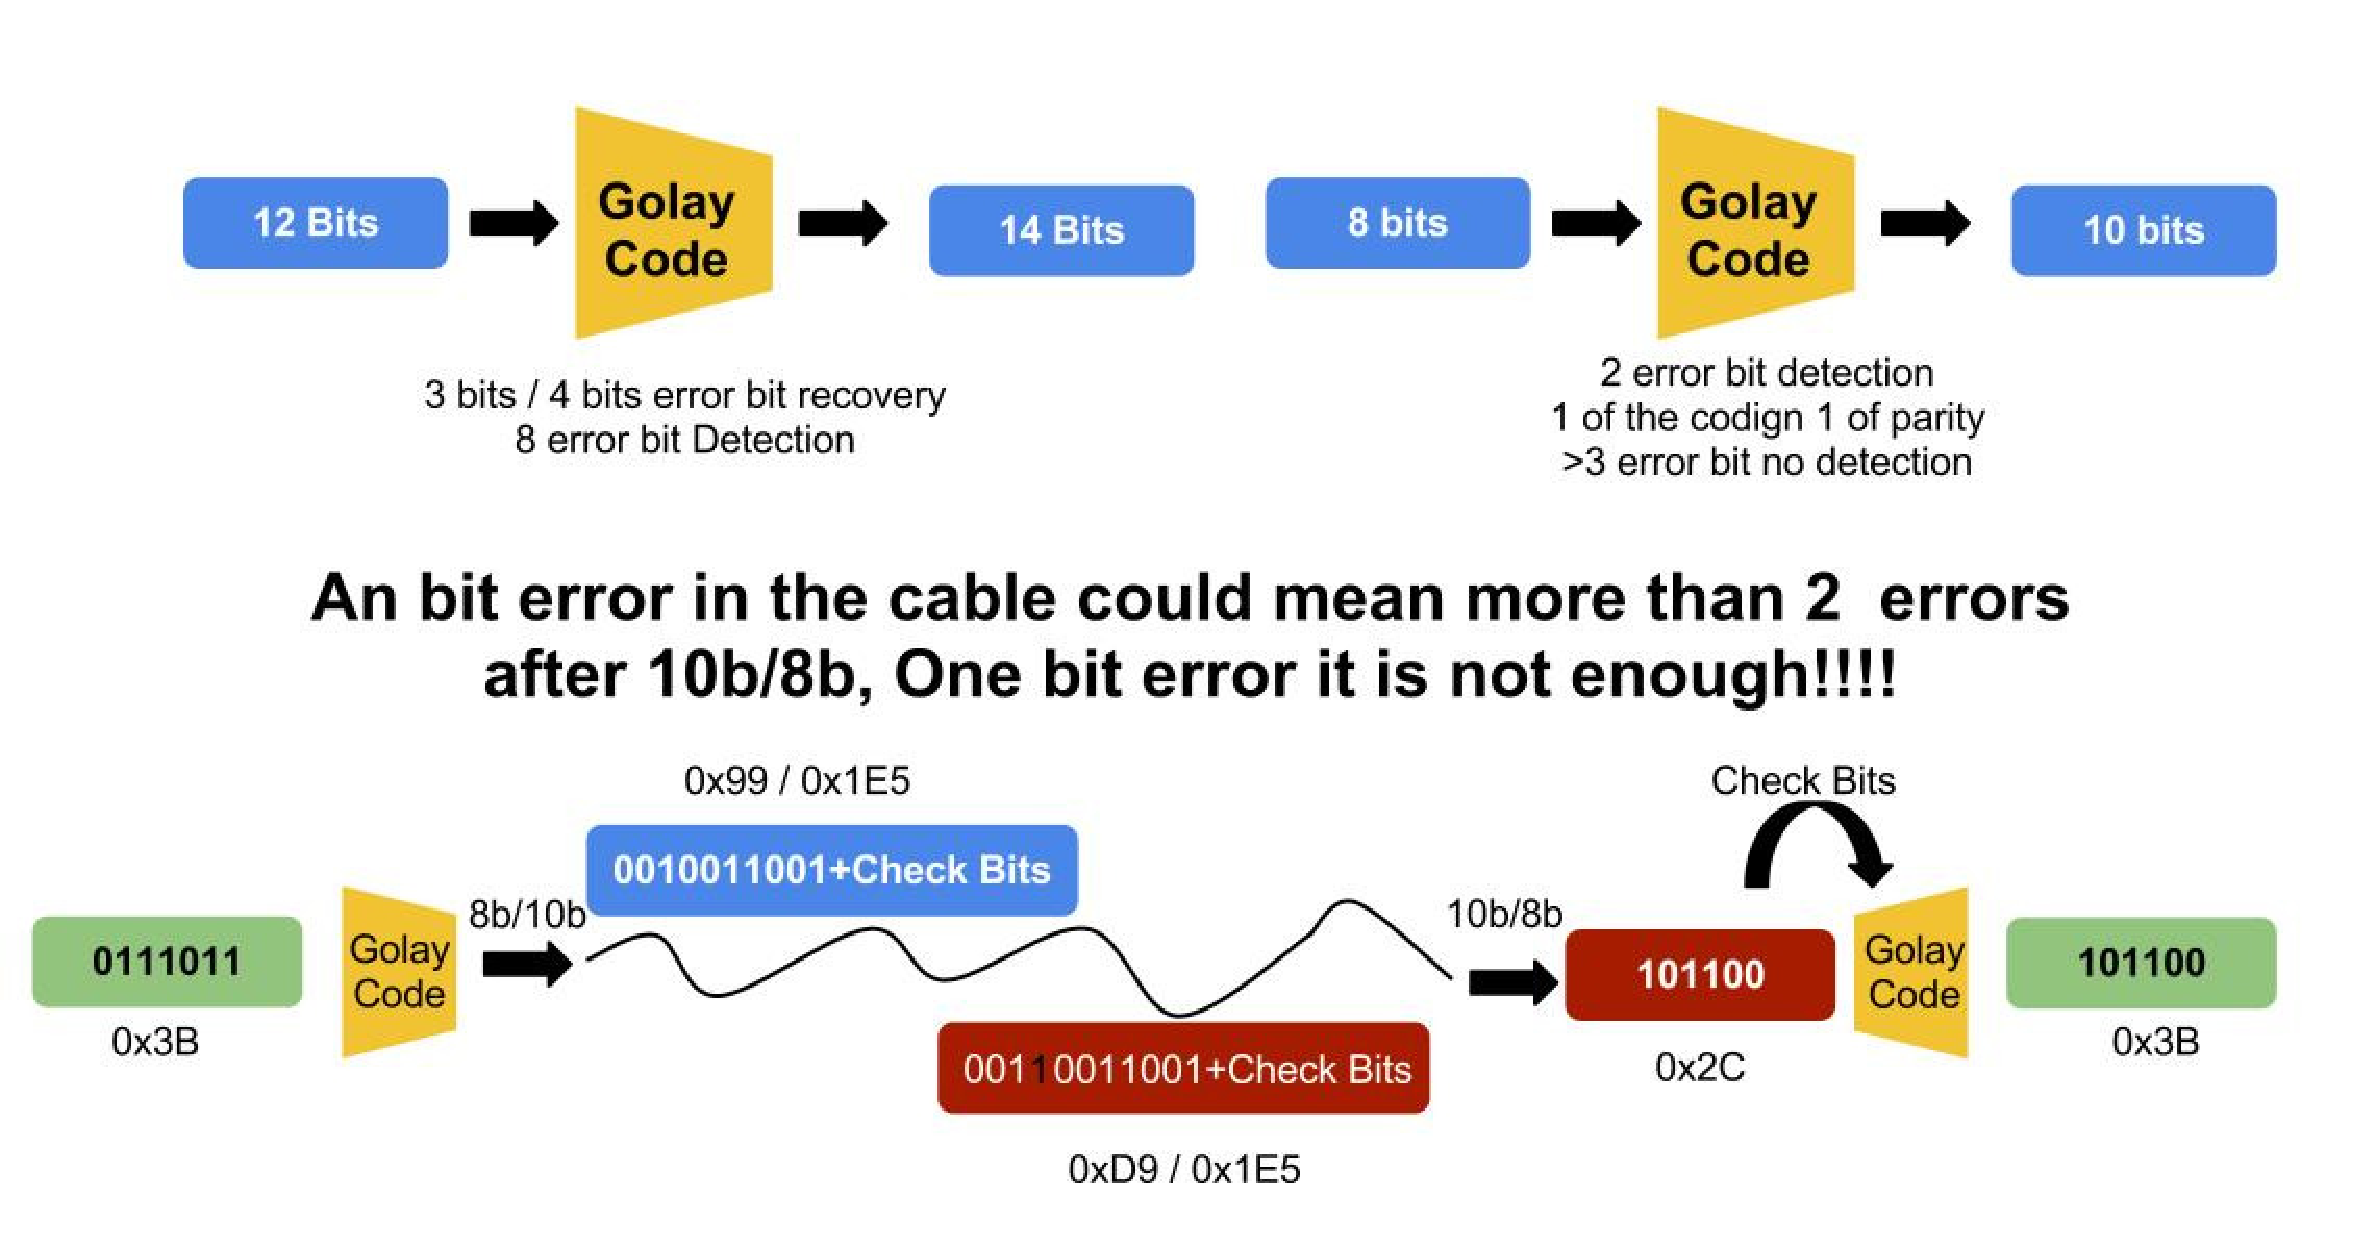
\includegraphics[scale=0.25]{../../figures/robustness/8b_10b_Golay.ps}
 \end{center}

\end{frame}

\begin{frame}{FEC: Linear Code and 8b/10b III}
    \begin{itemize}
        \item Golay is a (24,12,8) code, rate of $50\%$ 
        \item \textbf{Fixed encoding time} and \textbf{upper bound} for the
        \textbf{decoding}
        \item Hardware implementation of a variant of the Golay Code:
            \begin{itemize}
                \item Encoding in one clock
                \item Decoding, best case 2 clocks, worst case 6 clocks working
                at 125 Mhz 
            \end{itemize}
        \item Next steps: 
            \begin{itemize}
                \item hook it to the Starter Kit and plus the Block Code,
                and then we have a FEC.
                \item Customization of the code for our case 
            \end{itemize}
    \end{itemize}
\end{frame}
%%%%%%%%%%%%%%%%%%%%%%%%%%%%%%%%%%%%%%%%%%%%%%%%%%%%%%%%%%%%%%%%%%%%%%%%%%%%%%%%%%%%%%%%%%%%%%%%%%%%
\section{Topology}
\subsection{}
%%%%%%%%%%%%%%%%%%%%%%%%%%%%%%%%%%%%%%%%%%%%%%%%%%%%%%%%%%%%%%%%%%%%%%%%%%%%%%%%%%%%%%%%%%%%%%%%%%%%
\begin{frame}{Topology Redundancy}

      \begin{center}
	\includegraphics[width=.65\textwidth]{../../figures/network/WR_funny_network.ps}
      \end{center}

\end{frame}
%%%%%%%%%%%%%%%%%%%%%%%%%%%%%%%%%%%%%%%%%%%%%%%%%%%%%%%%%%%%%%%%%%%%%%%%%%%%%%%%%%%%%%%%%%%%%%%%%%%%
%\section{Topology}
%\subsection{}
%%%%%%%%%%%%%%%%%%%%%%%%%%%%%%%%%%%%%%%%%%%%%%%%%%%%%%%%%%%%%%%%%%%%%%%%%%%%%%%%%%%%%%%%%%%%%%%%%%%%
\begin{frame}{Topology Resolution}

  \begin{itemize}
    \item Target: $\leq$ 2 Ethernet Frames lost @ convergence
    \item Extensive research of current solutions
    \item Two solutions considered
    \begin{itemize}
      \item \textcolor{red}{enhanced Spanning Tree Protocol (WR STP)}
      \item \textcolor{red}{enhanced Link Aggregation Control Protocol (WR LACP)}
    \end{itemize}
    \item {\bf Universal firmware} to support enhancements
  \end{itemize}

      \begin{center}
	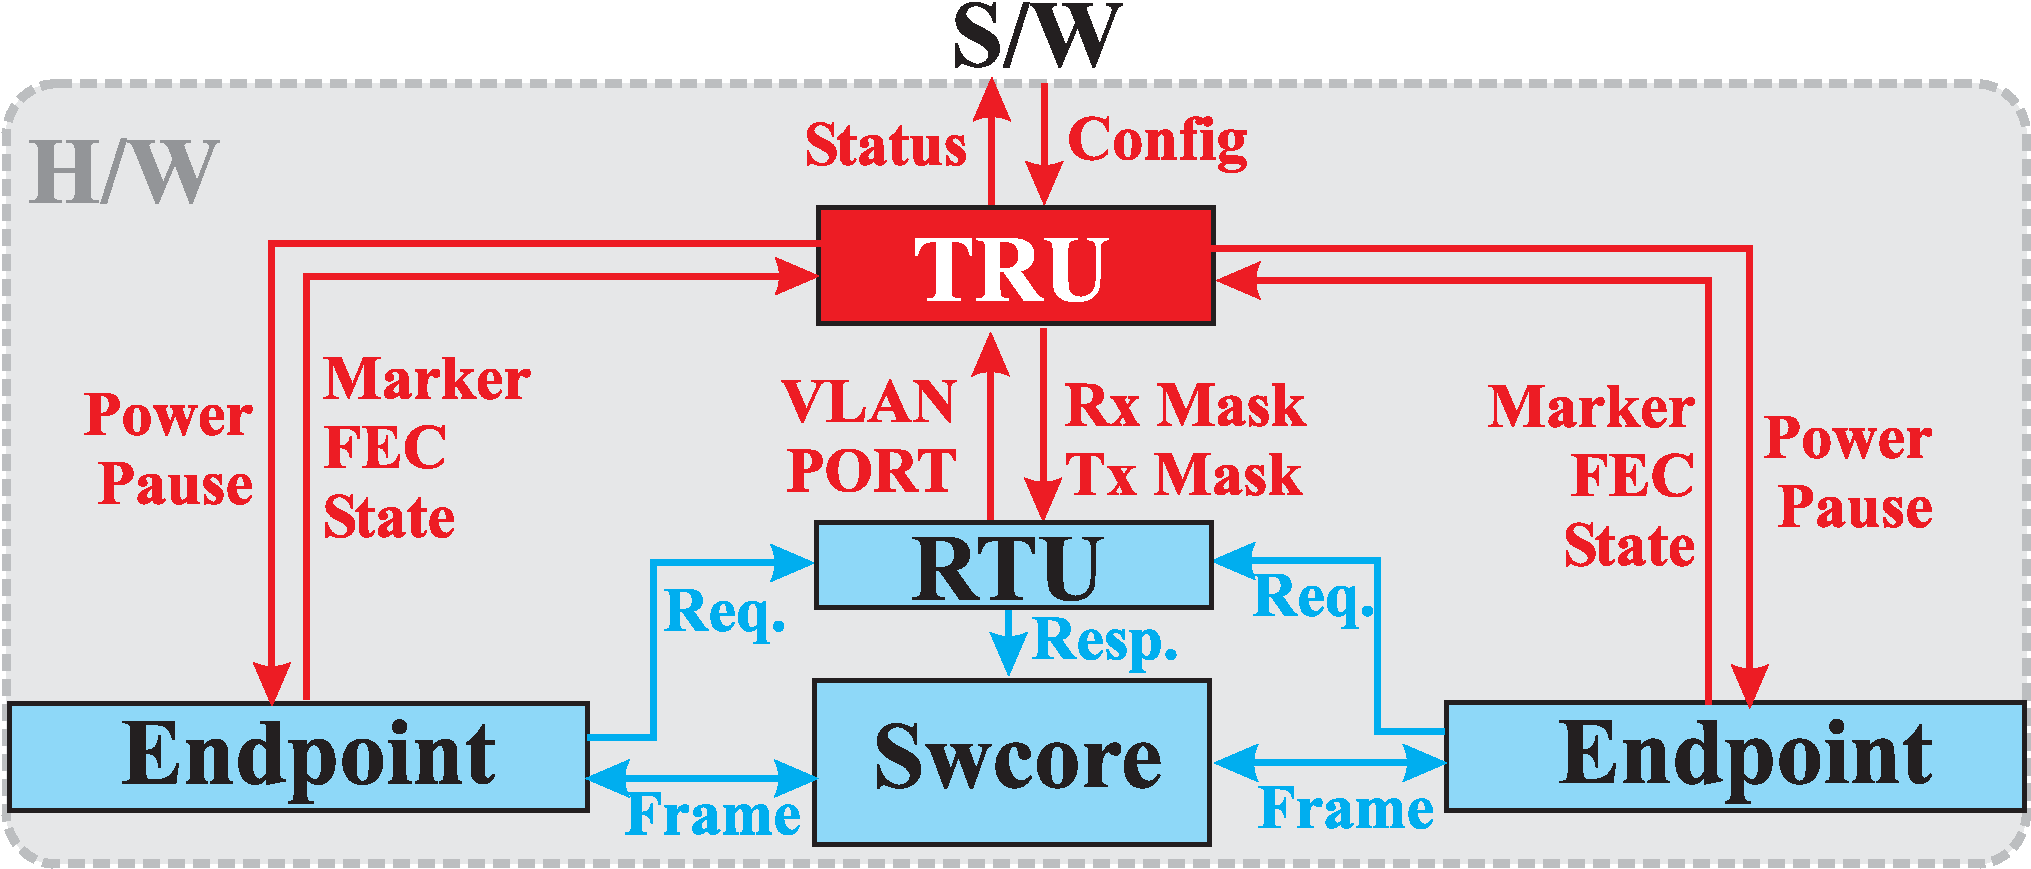
\includegraphics[width=.9\textwidth]{../../figures/robustness/TopologyResolutionUnit.eps}
      \end{center}

\end{frame}

%%%%%%%%%%%%%%%%%%%%%%%%%%%%%%%%%%%%%%%%%%%%%%%%%%%%%%%%%%%%%%%%%%%%%%%%%%%%%%%%%%%%%%%%%%%%%%%%%%%%
%\section{Topology}
% \subsection{Quality of Service}
%%%%%%%%%%%%%%%%%%%%%%%%%%%%%%%%%%%%%%%%%%%%%%%%%%%%%%%%%%%%%%%%%%%%%%%%%%%%%%%%%%%%%%%%%%%%%%%%%%%%
\begin{frame}{enhanced Spanning Tree Protocol}

\begin{columns}[c]
  \column{.65\textwidth}

  \begin{itemize}
    \item Ultra-fast convergence ($\approx$ 3 $\mu s$)
    \item Modification of Multiple/Rapid STP 
    \begin{itemize}
      \item hardware support
      \item software support
     \end{itemize}
    \item Basic concept  
\includegraphics[width=.5cm]{../../figures/misc/big-tick.ps}
    \item Implementation 
\includegraphics[width=.5cm]{../../figures/misc/underconstruction.ps}
  \end{itemize}

 \column{.35\textwidth}

      \begin{center}
	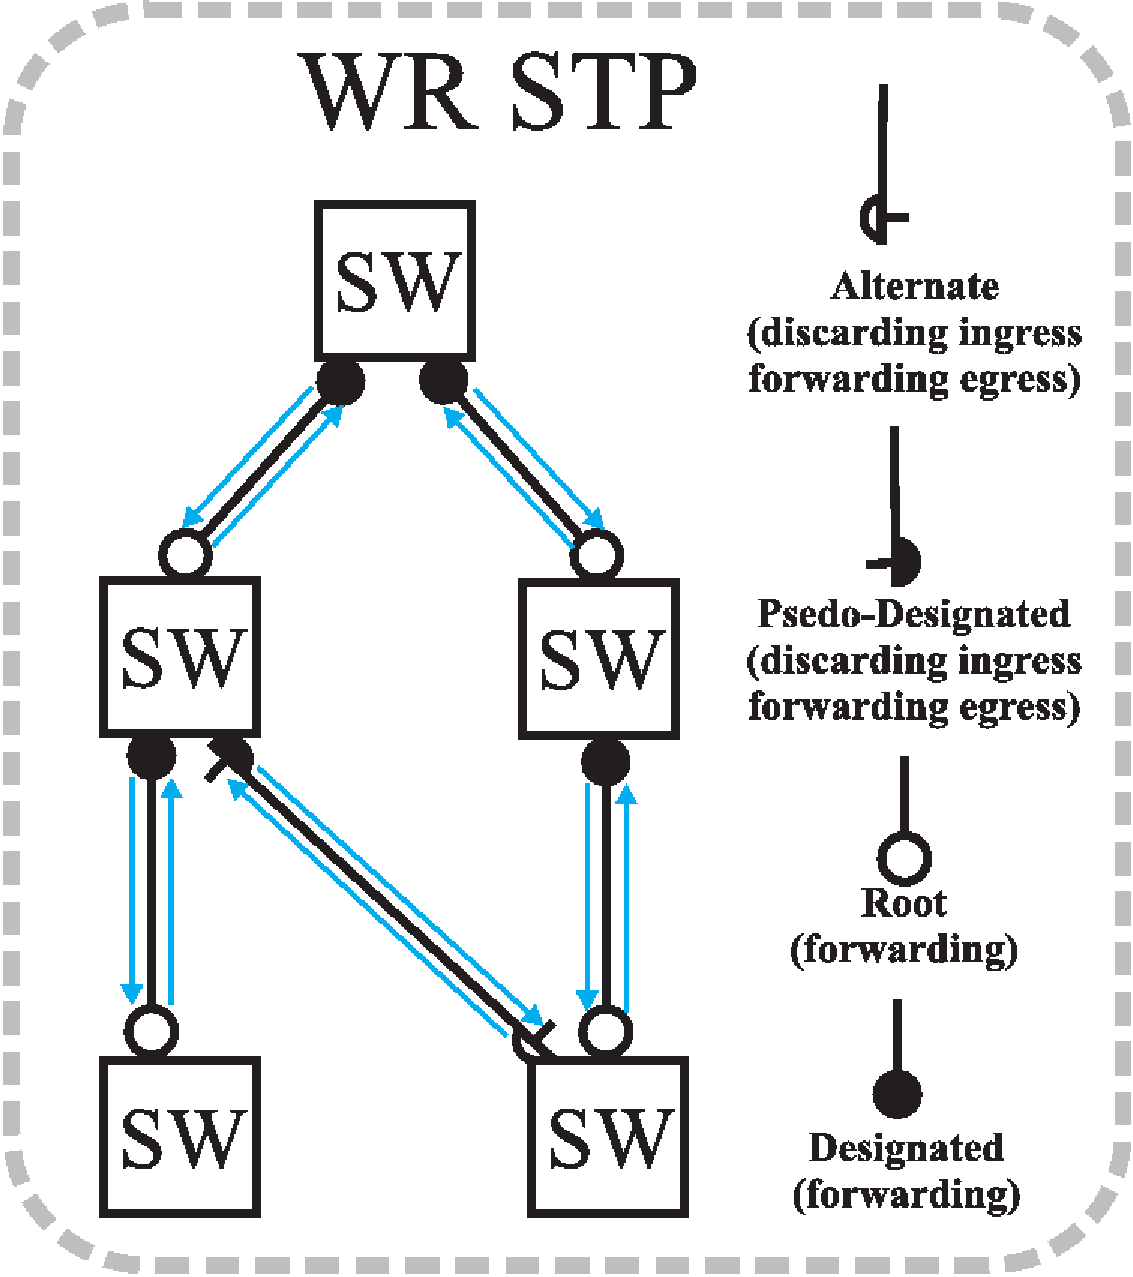
\includegraphics[width=1.1\textwidth]{../../figures/robustness/portRoles.v2.eps}
      \end{center}

 \end{columns}

\end{frame}

%%%%%%%%%%%%%%%%%%%%%%%%%%%%%%%%%%%%%%%%%%%%%%%%%%%%%%%%%%%%%%%%%%%%%%%%%%%%%%%%%%%%%%%%%%%%%%%%%%%%
%\section{Topology}
% \subsection{Quality of Service}
%%%%%%%%%%%%%%%%%%%%%%%%%%%%%%%%%%%%%%%%%%%%%%%%%%%%%%%%%%%%%%%%%%%%%%%%%%%%%%%%%%%%%%%%%%%%%%%%%%%%
\begin{frame}{Link Aggregation Control Protocol plus FEC I}

\begin{itemize}
    \item LACP provides the means to show two networks interface as a single  interfacea
    \item When the network interfaces are not in the same physical switch a  multipath is created for a frame
    \item Normally the multipath is used for balancing the traffic
    \item On the other hand, the FEC destributes the control information in several frames
    \item What if we send $X\%$ of this frames in one path and $Y\%$ in the alternative path
    \item We could overcome with sucseed single points of failure in the network: switch breakdown and damaged fiber optic or ports.
\end{itemize}
\end{frame}

%%%%%%%%%%%%%%%%%%%%%%%%%%%%%%%%%%%%%%%%%%%%%%%%%%%%%%%%%%%%%%%%%%%%%%%%%%%%%%%%%%%%%%%%%%%%%%%%%%%%
\begin{frame}{Link Aggregation Control Protocol plus FEC II}

      \begin{center}
	        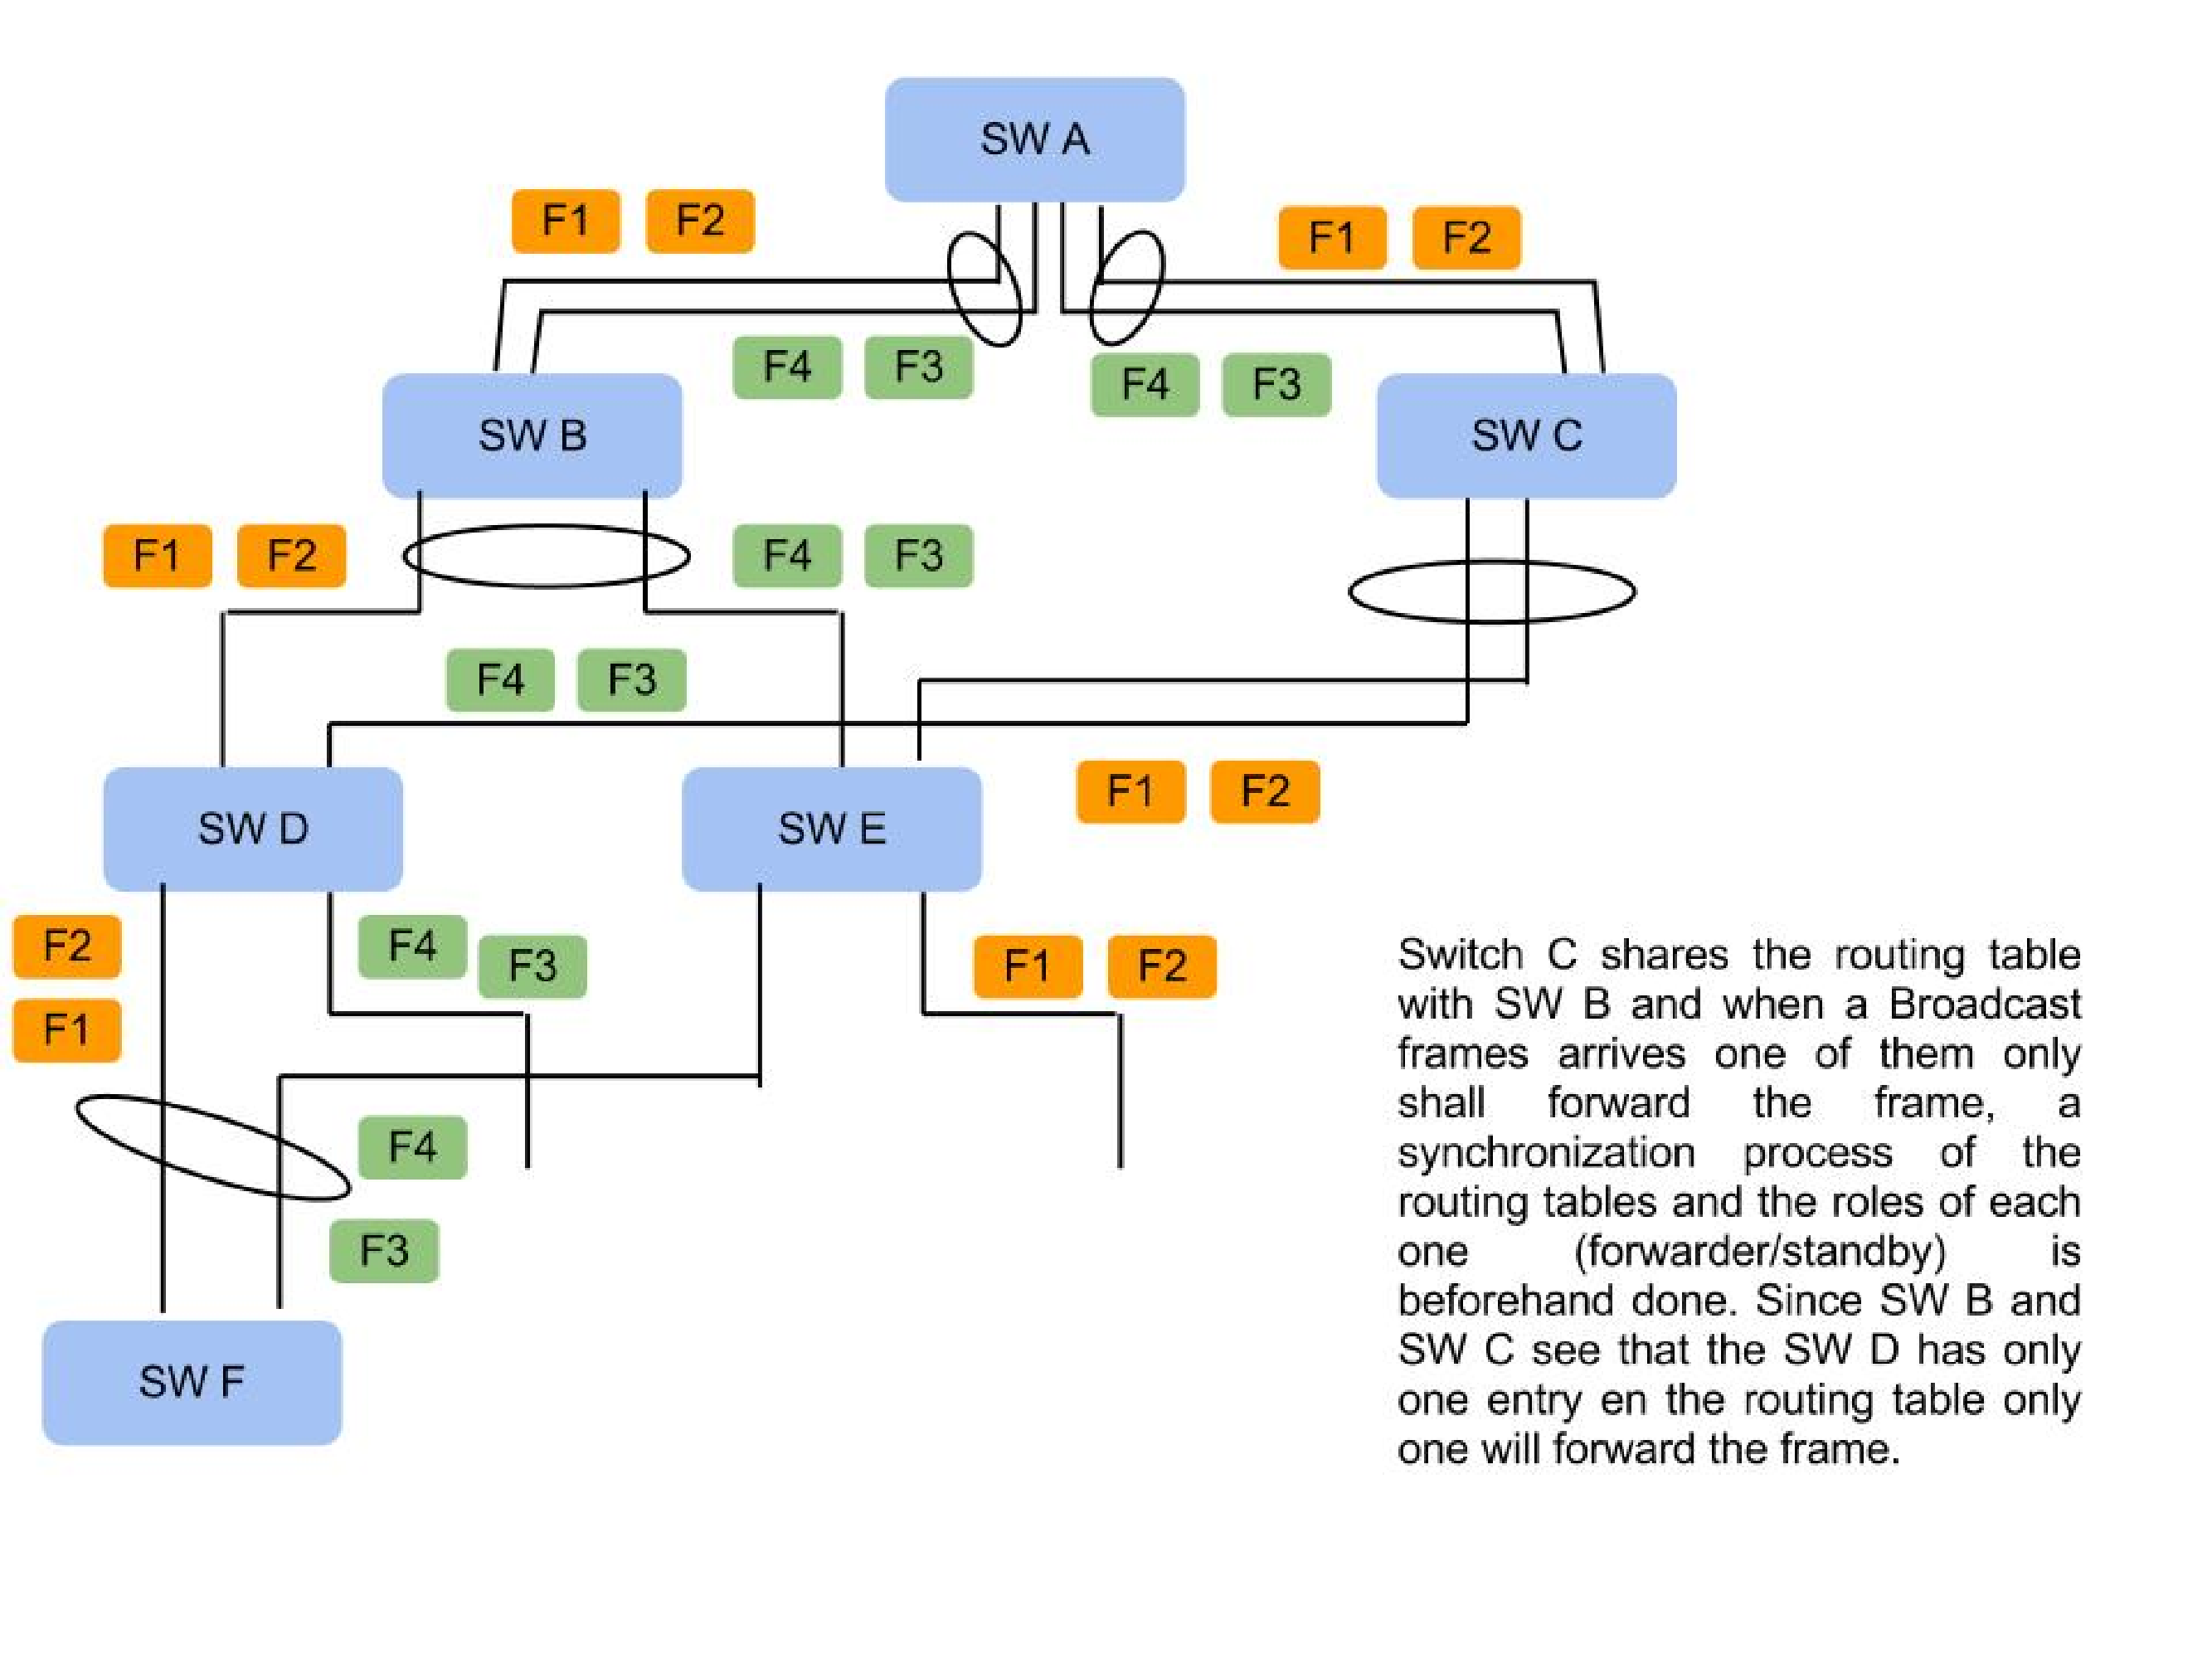
\includegraphics[scale=0.30]{../../figures/robustness/WR_LA_3.ps}
      \end{center}
\end{frame}


%%%%%%%%%%%%%%%%%%%%%%%%%%%%%%%%%%%%%%%%%%%%%%%%%%%%%%%%%%%%%%%%%%%%%%%%%%%%%%%%%%%%%%%%%%%%%%%%%%%%
\begin{frame}{Link Aggregation Control Protocol plus FEC III}

\begin{itemize}
    \item It fullfils the GSI and CERN 
    \item Doesn't jepardize the deterministic delivery of information, 
\end{itemize}

There is a smoothly continuation of the service there is not rush we have the \textbf{redundancy beforhand.}

Pros of LAC-FEC

\begin{itemize}
    \item There is not idle resources: port, fiber optic etc...
    \item At least duplication of the bandwidth upstream 
    \item The proposed scheme doesn't break the standard
    \item The IEEE standard is alive, present in almost all comercial switches (cisco, hp...)
\end{itemize}

\end{frame}


%%%%%%%%%%%%%%%%%%%%%%%%%%%%%%%%%%%%%%%%%%%%%%%%%%%%%%%%%%%%%%%%%%%%%%%%%%%%%%%%%%%%%%%%%%%%%%%%%%%%
\section{Networks}
\subsection{}
%%%%%%%%%%%%%%%%%%%%%%%%%%%%%%%%%%%%%%%%%%%%%%%%%%%%%%%%%%%%%%%%%%%%%%%%%%%%%%%%%%%%%%%%%%%%%%%%%%%%
\begin{frame}{WR@CERN: overview}


      \begin{center}
%	\includegraphics[width=1.0\textwidth]{fig/NT-overview.v2.eps}
	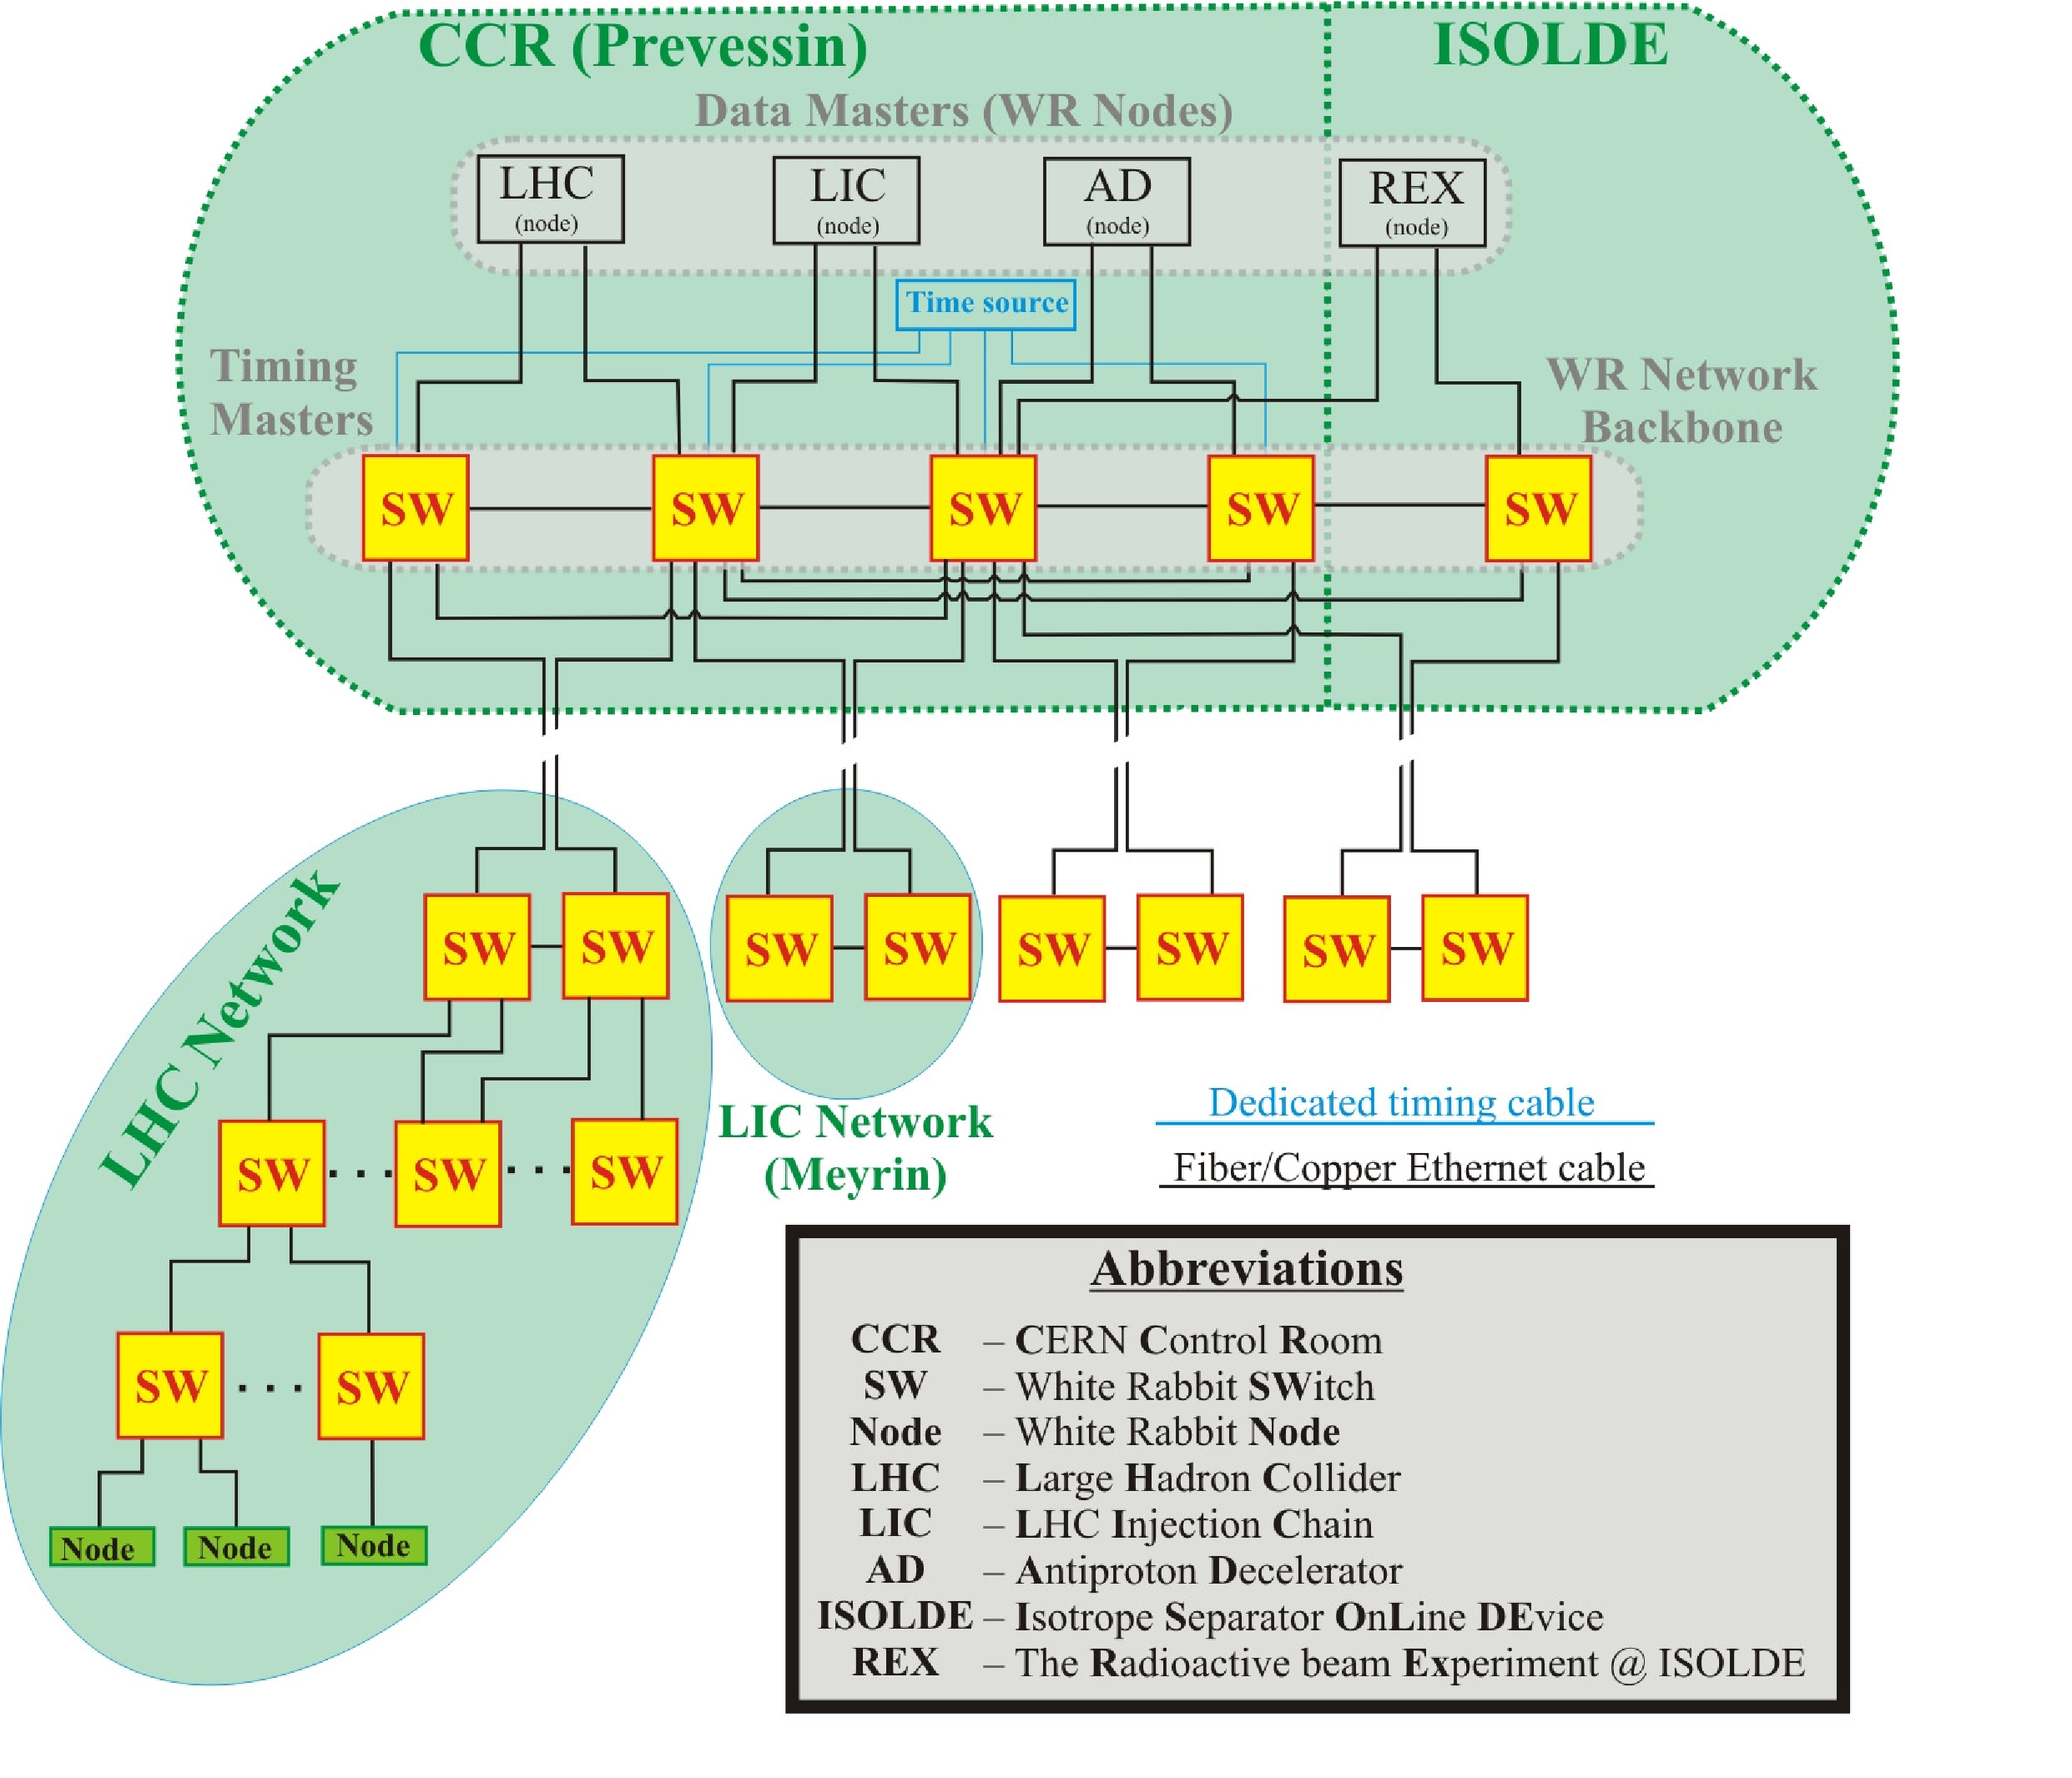
\includegraphics[width=0.8\textwidth]{../../figures/applications/CERN/NT-overview_legend.eps}
      \end{center}  

\end{frame}
%%%%%%%%%%%%%%%%%%%%%%%%%%%%%%%%%%%%%%%%%%%%%%%%%%%%%%%%%%%%%%%%%%%%%%%%%%%%%%%%%%%%%%%%%%%%%%%%%%%%
%\section{Networks}
% \subsection{Quality of Service}
%%%%%%%%%%%%%%%%%%%%%%%%%%%%%%%%%%%%%%%%%%%%%%%%%%%%%%%%%%%%%%%%%%%%%%%%%%%%%%%%%%%%%%%%%%%%%%%%%%%%
\begin{frame}{WR@CERN: VLANs}

      \begin{center}
	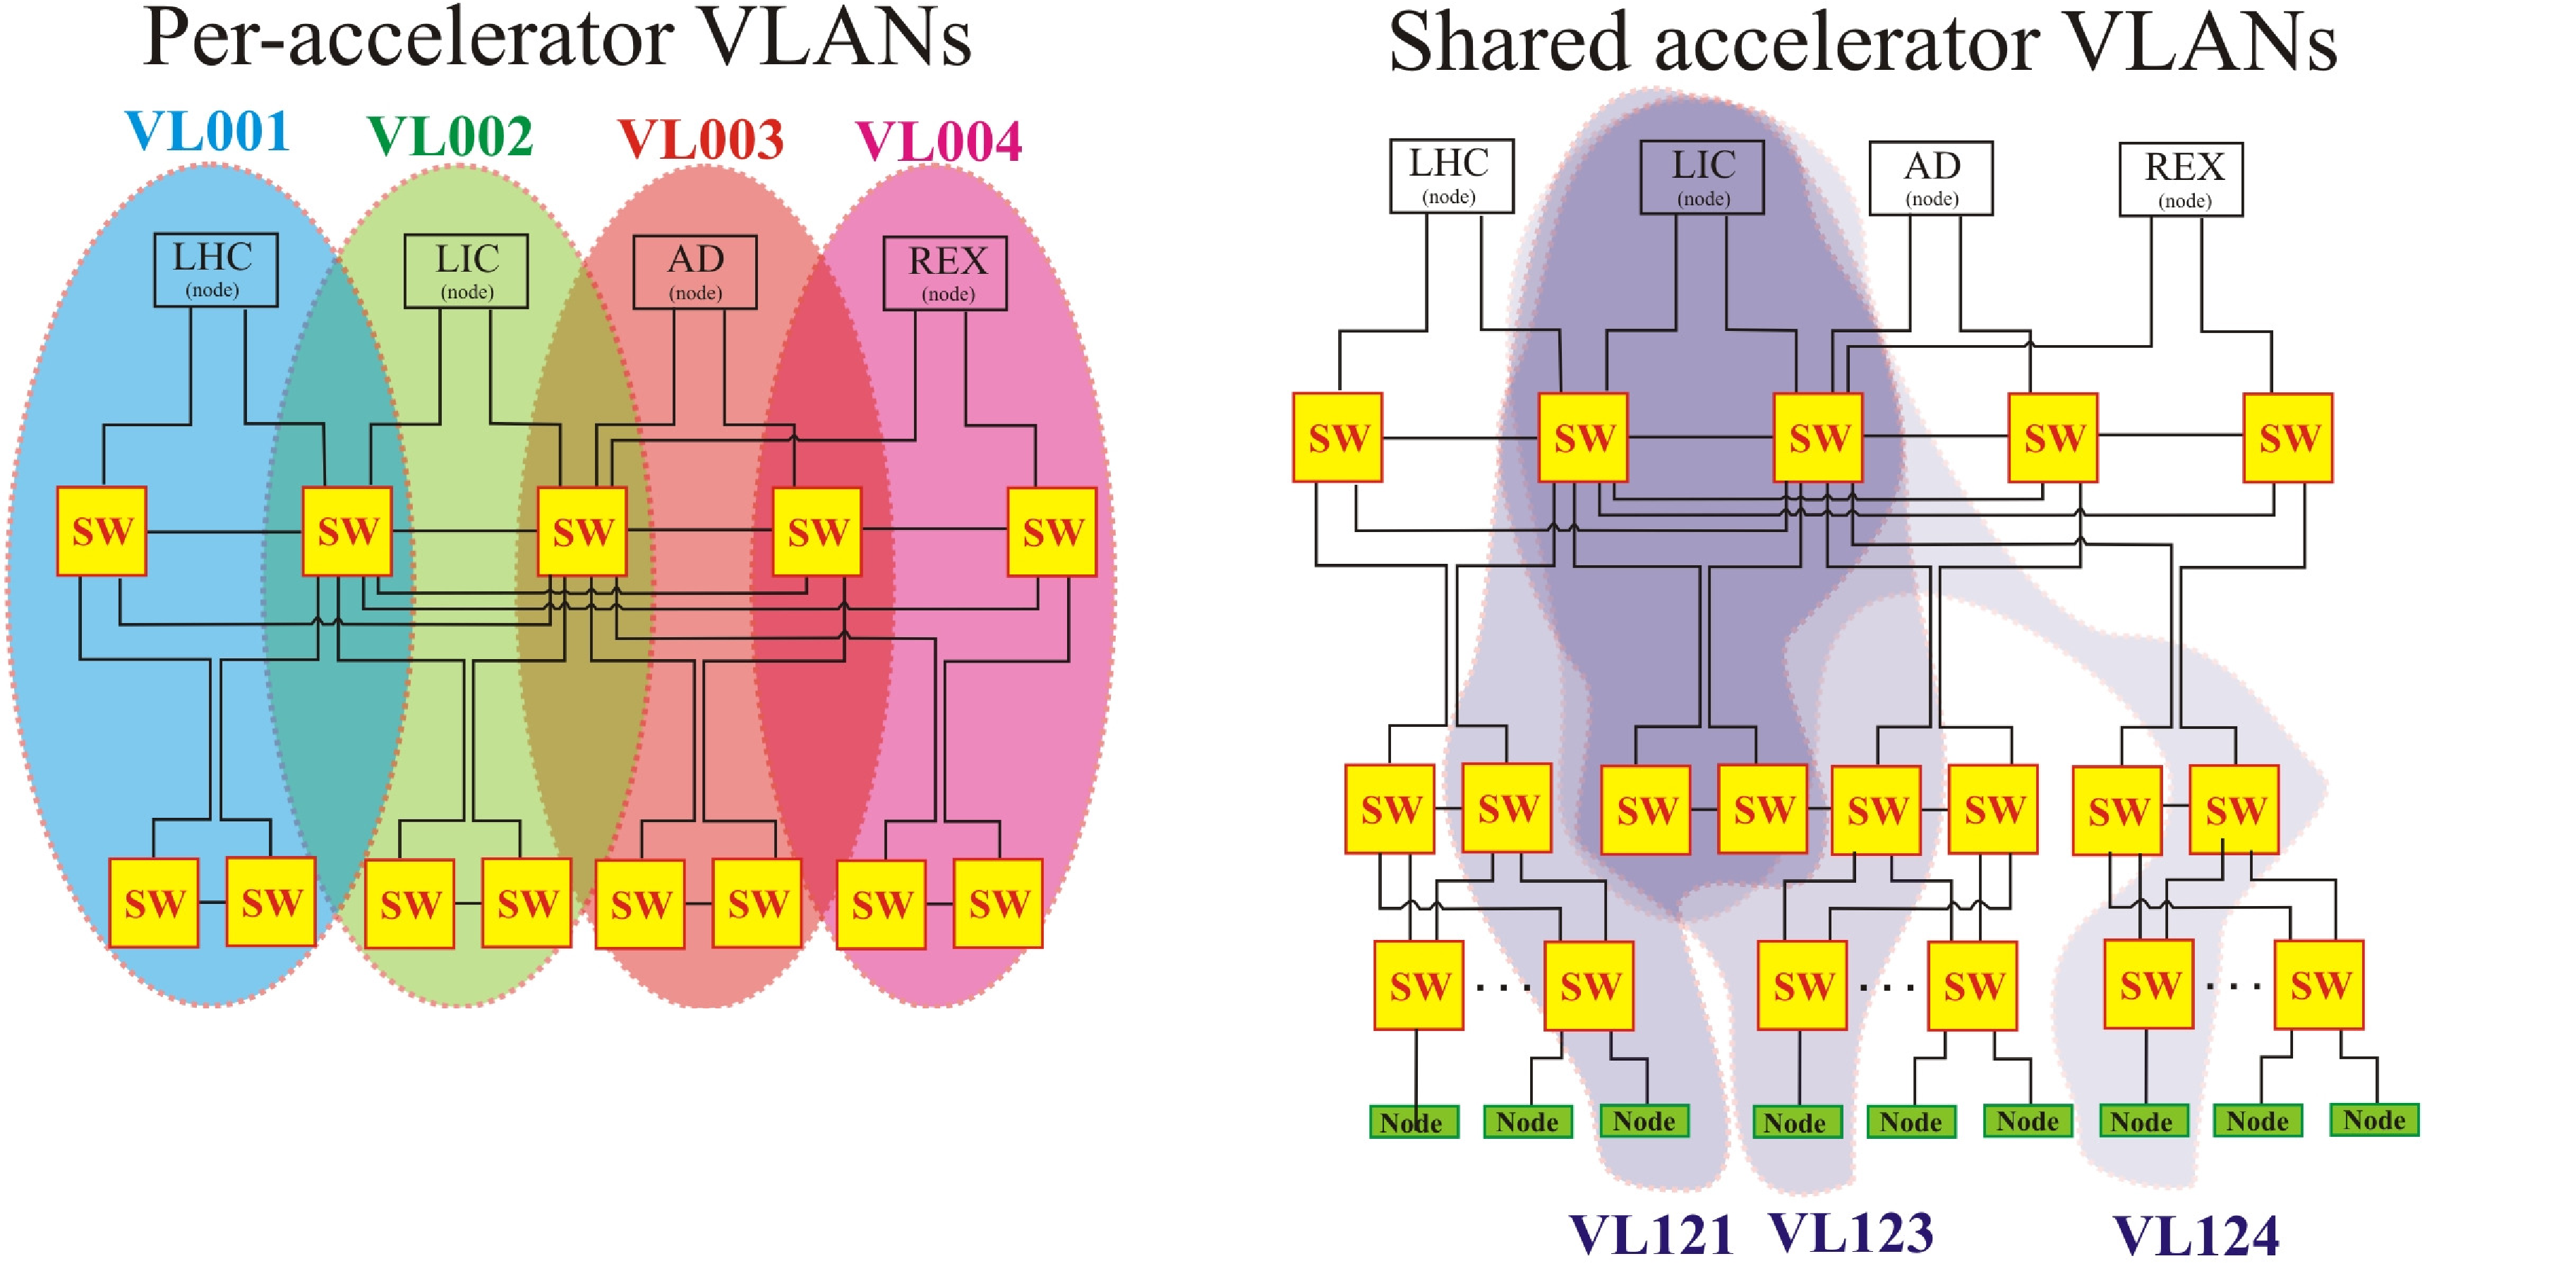
\includegraphics[width=1.1\textwidth]{../../figures/applications/CERN/NT-VLANs.v2.eps}
      \end{center}  

\end{frame}
%%%%%%%%%%%%%%%%%%%%%%%%%%%%%%%%%%%%%%%%%%%%%%%%%%%%%%%%%%%%%%%%%%%%%%%%%%%%%%%%%%%%%%%%%%%%%%%%%%%%
%\section{Networks}
% \subsection{Quality of Service}
%%%%%%%%%%%%%%%%%%%%%%%%%%%%%%%%%%%%%%%%%%%%%%%%%%%%%%%%%%%%%%%%%%%%%%%%%%%%%%%%%%%%%%%%%%%%%%%%%%%%
\begin{frame}{WR@CERN: Time distribution}


      \begin{center}
	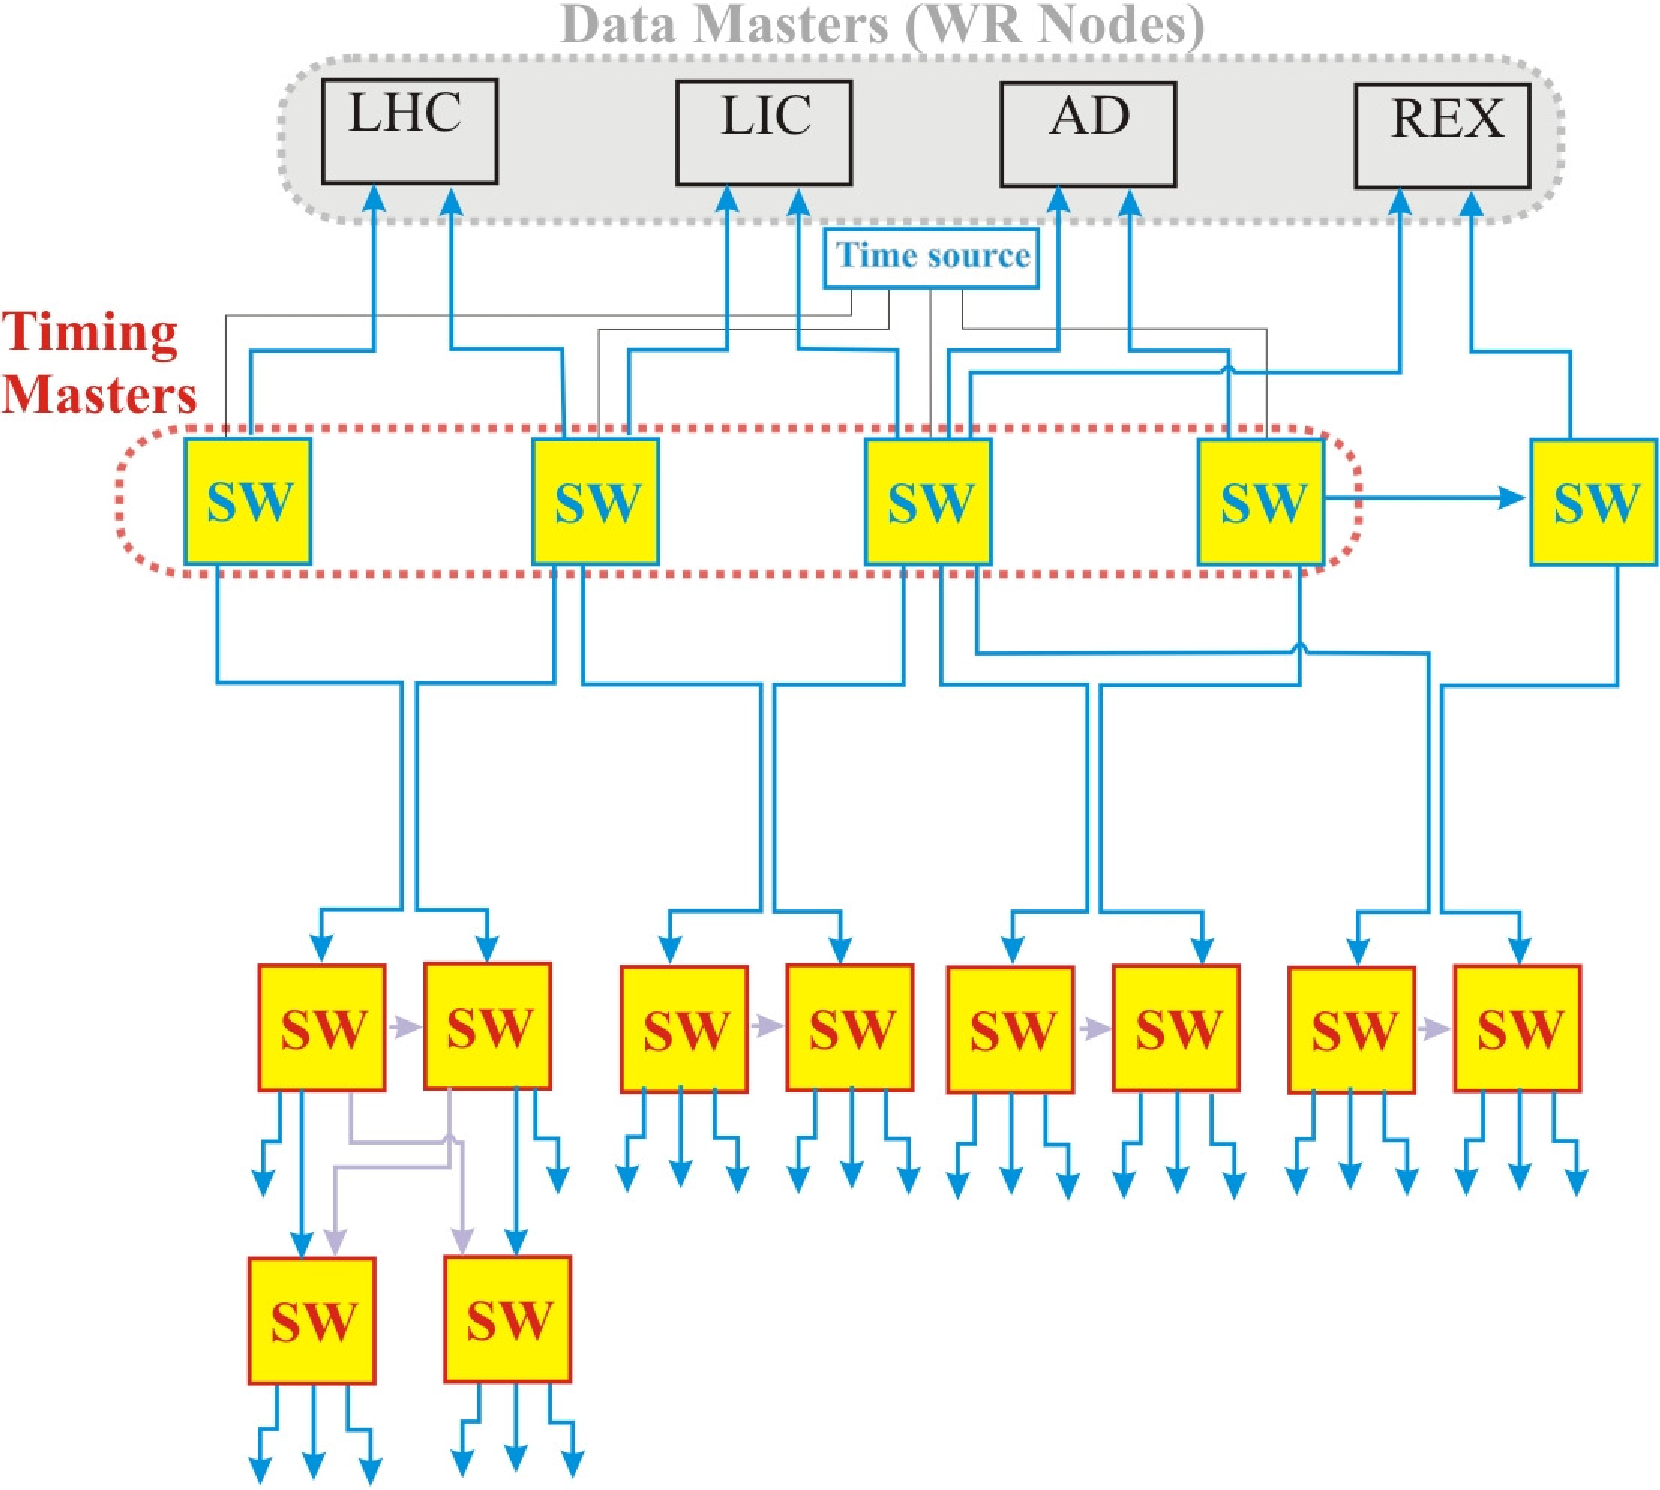
\includegraphics[width=.7\textwidth]{../../figures/applications/CERN/NT-timing.v2.eps}
      \end{center}  

\end{frame}

%%%%%%%%%%%%%%%%%%%%%%%%%%%%%%%%%%%%%%%%%%%%%%%%%%%%%%%%%%%%%%%%%%%%%%%%%%%%%%%%%%%%%%%%%%%%%%%%%%%%
%\section{Networks}
% \subsection{Quality of Service}
%%%%%%%%%%%%%%%%%%%%%%%%%%%%%%%%%%%%%%%%%%%%%%%%%%%%%%%%%%%%%%%%%%%%%%%%%%%%%%%%%%%%%%%%%%%%%%%%%%%%
\begin{frame}{WR@GSI: Overview}


      \begin{center}
	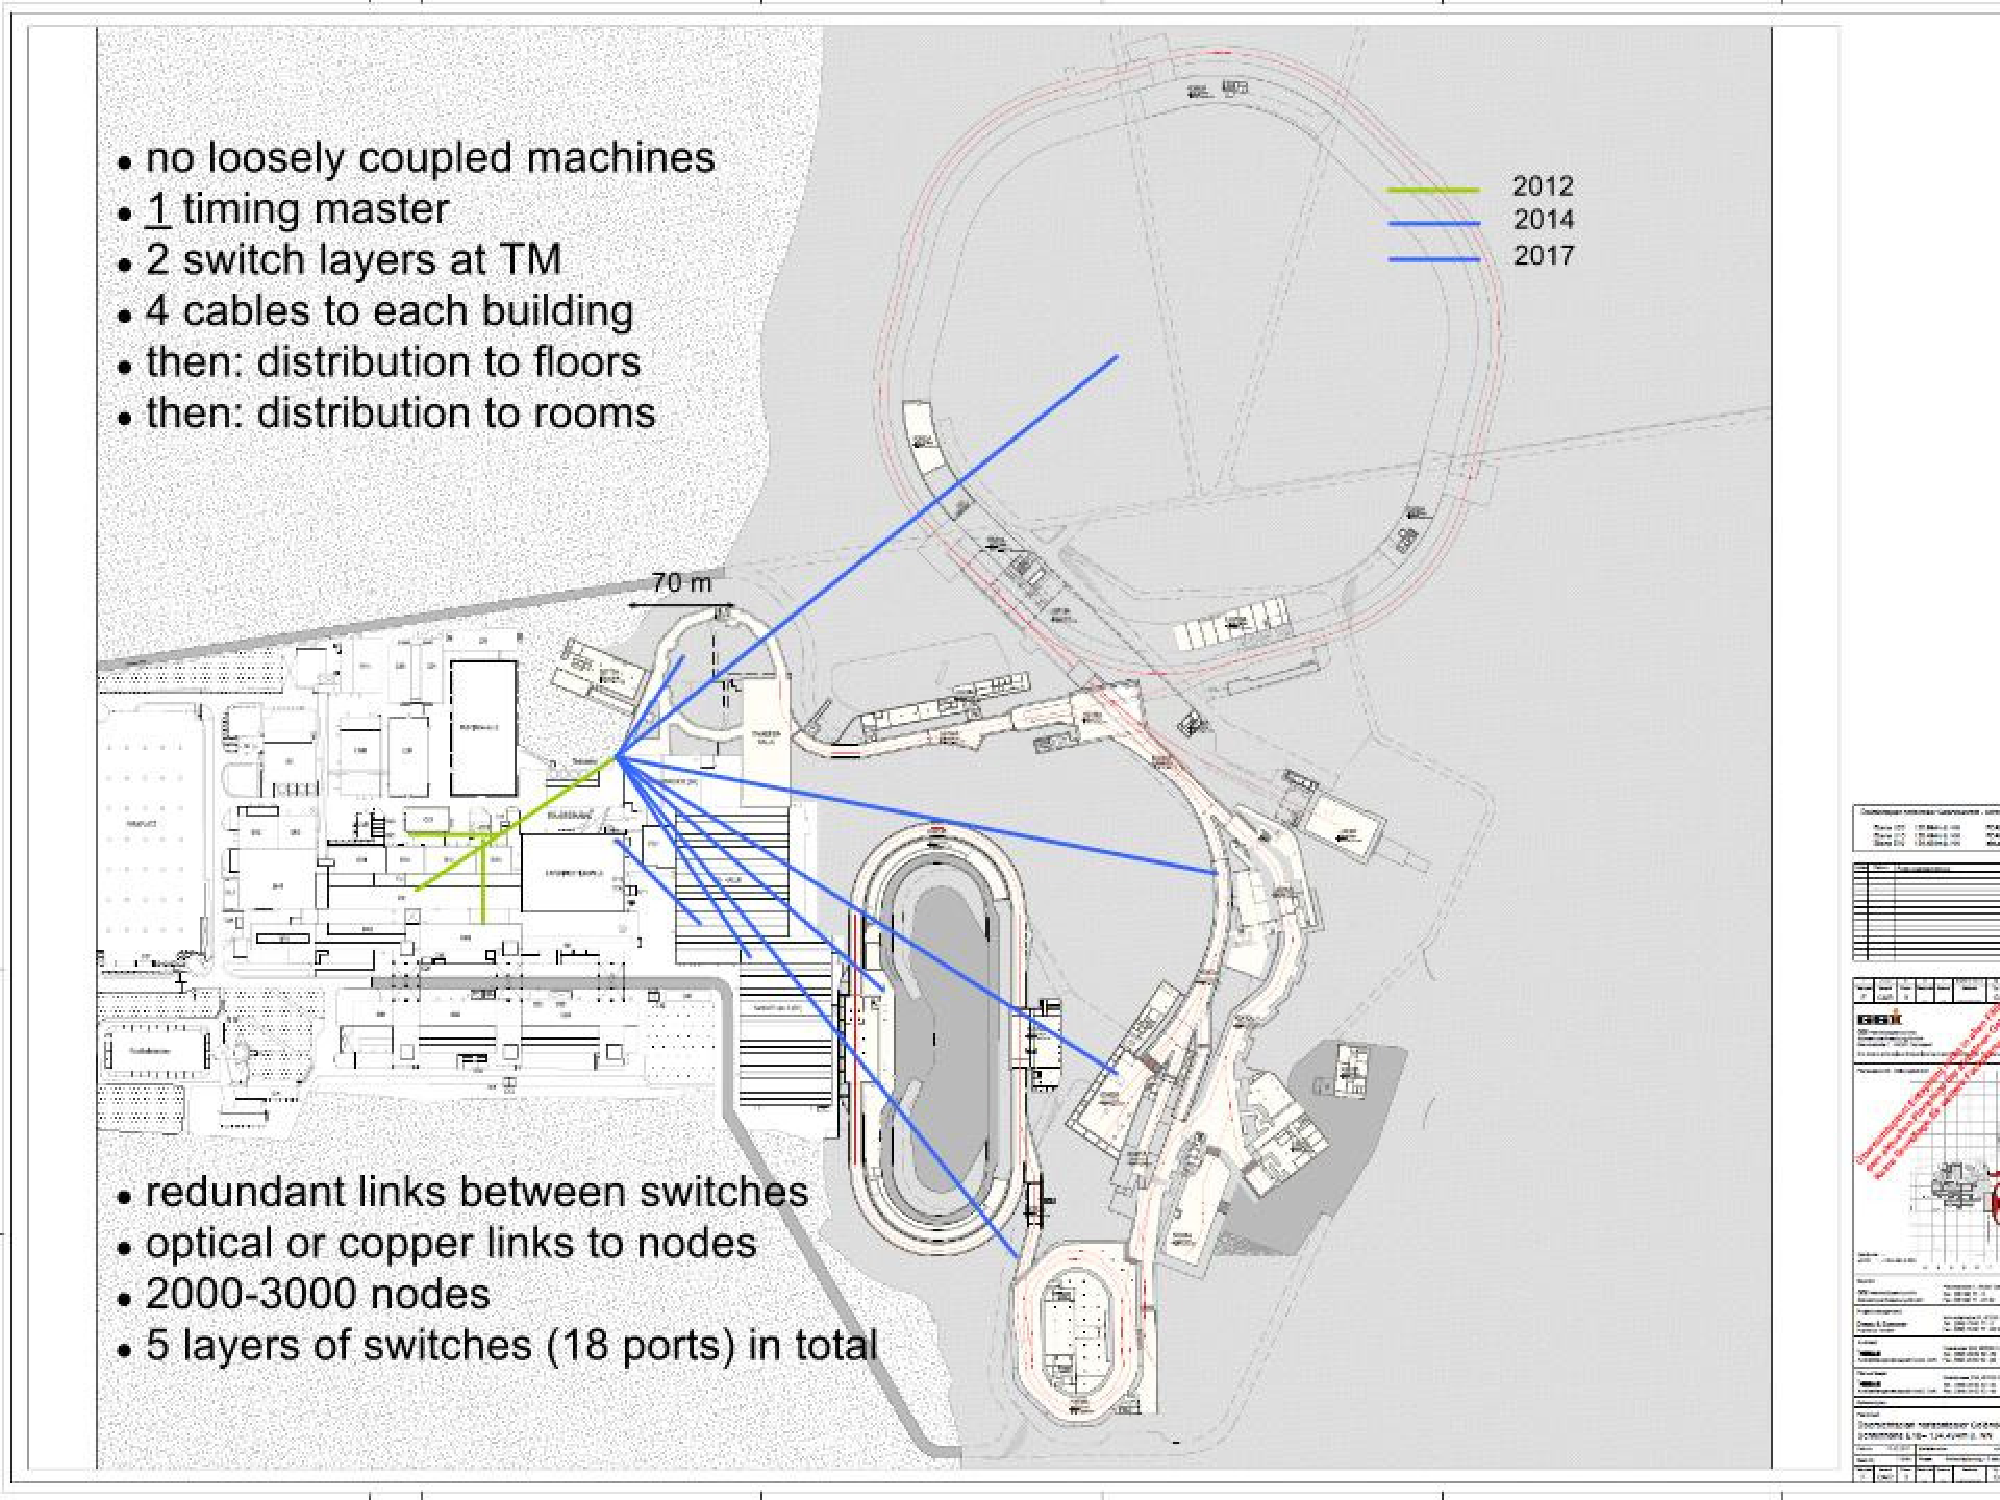
\includegraphics[scale=0.30]{../../figures/applications/gmt-at--fair.ppt.ps}
      \end{center}  

\end{frame}



%%%%%%%%%%%%%%%%%%%%%%%%%%%%%%%%%%%%%%%%%%%%%%%%%%%%%%%%%%%%%%%%%%%%%%%%%%%%%%%%%%%%%%%%%%%%%%%%%%%%
\section{Status and Plans}
\subsection{}
%%%%%%%%%%%%%%%%%%%%%%%%%%%%%%%%%%%%%%%%%%%%%%%%%%%%%%%%%%%%%%%%%%%%%%%%%%%%%%%%%%%%%%%%%%%%%%%%%%%%
\begin{frame}{Status}

%     Basic concept  
\includegraphics[width=.5cm]{../../figures/misc/big-tick.ps}
%     Implementation 
\includegraphics[width=.5cm]{../../figures/misc/underconstruction.ps}

\begin{columns}[c]
  \column{.5\textwidth}

    \begin{block}{{\bf Synchronization Resilience}}
      
\includegraphics[width=.5cm]{../../figures/misc/big-tick.ps}~~WRPTP support - improvements for further study \\
      
\includegraphics[width=.5cm]{../../figures/misc/underconstruction.ps}~~Hardware support
    \end{block}

    \begin{block}{{\bf Deterministic Packet Delivery}}
      
\includegraphics[width=.5cm]{../../figures/misc/big-tick.ps}~~Cut-through \\
      
\includegraphics[width=.5cm]{../../figures/misc/underconstruction.ps}~~Separate resources \\
      
\includegraphics[width=.5cm]{../../figures/misc/underconstruction.ps}~~Output queuing \\
      
\includegraphics[width=.5cm]{../../figures/misc/underconstruction.ps}~~Optimization
    \end{block}

  \column{.5\textwidth}
    \begin{block}{{\bf Data Resilience}}

      
\includegraphics[width=.5cm]{../../figures/misc/big-tick.ps}~~FEC Encoder - more work \\
      
\includegraphics[width=.5cm]{../../figures/misc/underconstruction.ps}~~FEC Decoder

    \end{block}

    \begin{block}{ {\bf Topology redundancy}}
      
\includegraphics[width=.5cm]{../../figures/misc/big-tick.ps}~~Extensive study \\
      
\includegraphics[width=.5cm]{../../figures/misc/underconstruction.ps}~~Hardware/software
    \end{block}

    \begin{block}{  {\bf Diagnostics}}
      
\includegraphics[width=.5cm]{../../figures/misc/underconstruction.ps}~~Software
    \end{block}

  \end{columns}


%   \begin{itemize}
%     \item {\bf Synchronization Resilience} \\
% 
%       
\includegraphics[width=.5cm]{../../figures/misc/big-tick.ps}~~WRPTP support - improvements for further study \\
%       
\includegraphics[width=.5cm]{../../figures/misc/underconstruction.ps}~~Hardware support
% 
%     \item {\bf Deterministic Packet Delivery} \\
% 
%       
\includegraphics[width=.5cm]{../../figures/misc/big-tick.ps}~~Cut-through \\
%       
\includegraphics[width=.5cm]{../../figures/misc/underconstruction.ps}~~Separate resources \\
%       
\includegraphics[width=.5cm]{../../figures/misc/underconstruction.ps}~~Output queuing \\
%       \includegraphics[width=.5cm]{../../figures/misc/underconstruction.ps}~~Optimization
% 
%     \item {\bf Data Resilience}\\
% 
%       \includegraphics[width=.5cm]{../../figures/misc/big-tick.ps}~~FEC Encoder - need more work \\
%       \includegraphics[width=.5cm]{../../figures/misc/underconstruction.ps}~~FEC Decoder
% 
%     \item {\bf Topology redundancy} \\
% 
%       \includegraphics[width=.5cm]{../../figures/misc/underconstruction.ps}~~Extensive study \\
%       \includegraphics[width=.5cm]{../../figures/misc/underconstruction.ps}~~Hardware/software
% 
%     \item {\bf Diagnostics} \includegraphics[width=.5cm]{../../figures/misc/underconstruction.ps}
%   \end{itemize}
\end{frame}

%%%%%%%%%%%%%%%%%%%%%%%%%%%%%%%%%%%%%%%%%%%%%%%%%%%%%%%%%%%%%%%%%%%%%%%%%%%%%%%%%%%%%%%%%%%%%%%%%%%%
% \section{Status and Plans}
% \subsection{Quality of Service}
%%%%%%%%%%%%%%%%%%%%%%%%%%%%%%%%%%%%%%%%%%%%%%%%%%%%%%%%%%%%%%%%%%%%%%%%%%%%%%%%%%%%%%%%%%%%%%%%%%%%
\begin{frame}{Plans (for the nearest future)}

  \begin{itemize}
    \item {\bf Synchronization Resilience}
    \begin{itemize}
      \item Hardware - implementation of switch-over
    \end{itemize}    
    \item {\bf Deterministic Packet Delivery}
    \begin{itemize}
      \item Hardware - re-implementation of Memory Management Unit
      \item Hardware - optimization of SWcore/RTU 
    \end{itemize}    
    \item {\bf Topology redundancy}
    \begin{itemize}
      \item Hardware - implementation of Topology Resolution Unit
      \item Hardware - modification of RTU 
      \item Software - implementation of daemon (PoC)
    \end{itemize}  
    \item {\bf Diagnostics} - software
  \end{itemize}
\end{frame}
%%%%%%%%%%%%%%%%%%%%%%%%%%%%%%%%%%%%%%%%%%%%%%%%%%%%%%%%%%%%%%%%%%%%%%%%%%%%%%%%%%%%%%%%%%%%%%%%%%%%
\section{}
\subsection{}
%%%%%%%%%%%%%%%%%%%%%%%%%%%%%%%%%%%%%%%%%%%%%%%%%%%%%%%%%%%%%%%%%%%%%%%%%%%%%%%%%%%%%%%%%%%%%%%%%%%%
\begin{frame}{Thank you}

%     \begin{center}
%     Any questions ?
%     \end{center}

    
    \begin{center}
    \includegraphics[height=6.0cm]{../../figures/logo/WRlogo.ps}
    \end{center}

\end{frame}

\end{document}
